%  LaTeX support: latex@mdpi.com 
%  For support, please attach all files needed for compiling as well as the log file, and specify your operating system, LaTeX version, and LaTeX editor.

%=================================================================
\documentclass[electronics,article,accept,pdftex,moreauthors]{Definitions/mdpi} 
\linenumbers
%--------------------
% Class Options:
%--------------------
%----------
% journal
%----------
% Choose between the following MDPI journals:
% acoustics, actuators, addictions, admsci, adolescents, aerobiology, aerospace, agriculture, agriengineering, agrochemicals, agronomy, ai, air, algorithms, allergies, alloys, analytica, analytics, anatomia, animals, antibiotics, antibodies, antioxidants, applbiosci, appliedchem, appliedmath, applmech, applmicrobiol, applnano, applsci, aquacj, architecture, arm, arthropoda, arts, asc, asi, astronomy, atmosphere, atoms, audiolres, automation, axioms, bacteria, batteries, bdcc, behavsci, beverages, biochem, bioengineering, biologics, biology, biomass, biomechanics, biomed, biomedicines, biomedinformatics, biomimetics, biomolecules, biophysica, biosensors, biotech, birds, bloods, blsf, brainsci, breath, buildings, businesses, cancers, carbon, cardiogenetics, catalysts, cells, ceramics, challenges, chemengineering, chemistry, chemosensors, chemproc, children, chips, cimb, civileng, cleantechnol, climate, clinpract, clockssleep, cmd, coasts, coatings, colloids, colorants, commodities, compounds, computation, computers, condensedmatter, conservation, constrmater, cosmetics, covid, crops, cryptography, crystals, csmf, ctn, curroncol, cyber, dairy, data, ddc, dentistry, dermato, dermatopathology, designs, devices, diabetology, diagnostics, dietetics, digital, disabilities, diseases, diversity, dna, drones, dynamics, earth, ebj, ecologies, econometrics, economies, education, ejihpe, electricity, electrochem, electronicmat, electronics, encyclopedia, endocrines, energies, eng, engproc, entomology, entropy, environments, environsciproc, epidemiologia, epigenomes, est, fermentation, fibers, fintech, fire, fishes, fluids, foods, forecasting, forensicsci, forests, foundations, fractalfract, fuels, future, futureinternet, futurepharmacol, futurephys, futuretransp, galaxies, games, gases, gastroent, gastrointestdisord, gels, genealogy, genes, geographies, geohazards, geomatics, geosciences, geotechnics, geriatrics, grasses, gucdd, hazardousmatters, healthcare, hearts, hemato, hematolrep, heritage, higheredu, highthroughput, histories, horticulturae, hospitals, humanities, humans, hydrobiology, hydrogen, hydrology, hygiene, idr, ijerph, ijfs, ijgi, ijms, ijns, ijpb, ijtm, ijtpp, ime, immuno, informatics, information, infrastructures, inorganics, insects, instruments, inventions, iot, j, jal, jcdd, jcm, jcp, jcs, jcto, jdb, jeta, jfb, jfmk, jimaging, jintelligence, jlpea, jmmp, jmp, jmse, jne, jnt, jof, joitmc, jor, journalmedia, jox, jpm, jrfm, jsan, jtaer, jvd, jzbg, kidneydial, kinasesphosphatases, knowledge, land, languages, laws, life, liquids, literature, livers, logics, logistics, lubricants, lymphatics, machines, macromol, magnetism, magnetochemistry, make, marinedrugs, materials, materproc, mathematics, mca, measurements, medicina, medicines, medsci, membranes, merits, metabolites, metals, meteorology, methane, metrology, micro, microarrays, microbiolres, micromachines, microorganisms, microplastics, minerals, mining, modelling, molbank, molecules, mps, msf, mti, muscles, nanoenergyadv, nanomanufacturing,\gdef\@continuouspages{yes}} nanomaterials, ncrna, ndt, network, neuroglia, neurolint, neurosci, nitrogen, notspecified, %%nri, nursrep, nutraceuticals, nutrients, obesities, oceans, ohbm, onco, %oncopathology, optics, oral, organics, organoids, osteology, oxygen, parasites, parasitologia, particles, pathogens, pathophysiology, pediatrrep, pharmaceuticals, pharmaceutics, pharmacoepidemiology,\gdef\@ISSN{2813-0618}\gdef\@continuous pharmacy, philosophies, photochem, photonics, phycology, physchem, physics, physiologia, plants, plasma, platforms, pollutants, polymers, polysaccharides, poultry, powders, preprints, proceedings, processes, prosthesis, proteomes, psf, psych, psychiatryint, psychoactives, publications, quantumrep, quaternary, qubs, radiation, reactions, receptors, recycling, regeneration, religions, remotesensing, reports, reprodmed, resources, rheumato, risks, robotics, ruminants, safety, sci, scipharm, sclerosis, seeds, sensors, separations, sexes, signals, sinusitis, skins, smartcities, sna, societies, socsci, software, soilsystems, solar, solids, spectroscj, sports, standards, stats, std, stresses, surfaces, surgeries, suschem, sustainability, symmetry, synbio, systems, targets, taxonomy, technologies, telecom, test, textiles, thalassrep, thermo, tomography, tourismhosp, toxics, toxins, transplantology, transportation, traumacare, traumas, tropicalmed, universe, urbansci, uro, vaccines, vehicles, venereology, vetsci, vibration, virtualworlds, viruses, vision, waste, water, wem, wevj, wind, women, world, youth, zoonoticdis 
% For posting an early version of this manuscript as a preprint, you may use "preprints" as the journal. Changing "submit" to "accept" before posting will remove line numbers.

%---------
% article
%---------
% The default type of manuscript is "article", but can be replaced by: 
% abstract, addendum, article, book, bookreview, briefreport, casereport, comment, commentary, communication, conferenceproceedings, correction, conferencereport, entry, expressionofconcern, extendedabstract, datadescriptor, editorial, essay, erratum, hypothesis, interestingimage, obituary, opinion, projectreport, reply, retraction, review, perspective, protocol, shortnote, studyprotocol, systematicreview, supfile, technicalnote, viewpoint, guidelines, registeredreport, tutorial
% supfile = supplementary materials

%----------
% submit
%----------
% The class option "submit" will be changed to "accept" by the Editorial Office when the paper is accepted. This will only make changes to the frontpage (e.g., the logo of the journal will get visible), the headings, and the copyright information. Also, line numbering will be removed. Journal info and pagination for accepted papers will also be assigned by the Editorial Office.

%------------------
% moreauthors
%------------------
% If there is only one author the class option oneauthor should be used. Otherwise use the class option moreauthors.

%---------
% pdftex
%---------
% The option pdftex is for use with pdfLaTeX. Remove "pdftex" for (1) compiling with LaTeX & dvi2pdf (if eps figures are used) or for (2) compiling with XeLaTeX.

%=================================================================
% MDPI internal commands - do not modify
\firstpage{1} 
\makeatletter 
\setcounter{page}{\@firstpage} 
\makeatother
\pubvolume{1}
\issuenum{1}
\articlenumber{0}
\pubyear{2024}
\copyrightyear{2024}
%\externaleditor{Academic Editor: Firstname Lastname}
\datereceived{ } 
\daterevised{ } % Comment out if no revised date
\dateaccepted{ } 
\datepublished{ } 
%\datecorrected{} % For corrected papers: "Corrected: XXX" date in the original paper.
%\dateretracted{} % For corrected papers: "Retracted: XXX" date in the original paper.
\hreflink{https://doi.org/} % If needed use \linebreak
%\doinum{}
%\pdfoutput=1 % Uncommented for upload to arXiv.org
%\CorrStatement{yes}  % For updates
\usepackage{float}
% \usepackage{pifont}
% \newcommand{\circled}[1]{\ding{\numexpr171+#1\relax}}

\usepackage{tikz}
\usepackage{graphicx} % For \resizebox
\usepackage{diagbox} % For diagonal boxes
\usepackage{amsmath} % For math symbols
\usepackage{array} % For column formatting

\newcommand{\circled}[1]{%
    \tikz[baseline=(char.base)]{%
        \node[circle,draw,inner sep=0.5pt] (char) {\small #1};%
    }%
}

%\usepackage[backend=biber, style=numeric, sorting=none]{biblatex}
%
%\bibliography{references.bib}
%\DeclareFieldFormat*{parens}{#1\addperiod\addspace}
\usepackage{graphicx}
\usepackage{subcaption}
\renewcommand{\thesubfigure}{\arabic{subfigure}} % 子图序号使用阿拉伯数字
%=================================================================
% Add packages and commands here. The following packages are loaded in our class file: fontenc, inputenc, calc, indentfirst, fancyhdr, graphicx, epstopdf, lastpage, ifthen, float, amsmath, amssymb, lineno, setspace, enumitem, mathpazo, booktabs, titlesec, etoolbox, tabto, xcolor, colortbl, soul, multirow, microtype, tikz, totcount, changepage, attrib, upgreek, array, tabularx, pbox, ragged2e, tocloft, marginnote, marginfix, enotez, amsthm, natbib, hyperref, cleveref, scrextend, url, geometry, newfloat, caption, draftwatermark, seqsplit
% cleveref: load \crefname definitions after \begin{document}

%=================================================================
% Please use the following mathematics environments: Theorem, Lemma, Corollary, Proposition, Characterization, Property, Problem, Example, ExamplesandDefinitions, Hypothesis, Remark, Definition, Notation, Assumption
%% For proofs, please use the proof environment (the amsthm package is loaded by the MDPI class).

%=================================================================
% Full title of the paper (Capitalized)
\Title{Research on Multiplication Routines Based on Reconfigurable Four-Valued Logic Processor}

% MDPI internal command: Title for citation in the left column
\TitleCitation{Research on Multiplication Routines Based on Reconfigurable Four-Valued Logic Processor}

% Author Orchid ID: enter ID or remove command
\newcommand{\orcidauthorA}{0000-0000-0000-000X} % Add \orcidA{} behind the author's name
%\newcommand{\orcidauthorB}{0000-0000-0000-000X} % Add \orcidB{} behind the author's name

% Authors, for the paper (add full first names)

\Author{Shanchuan Liao $^{1}$\orcidA{}, Shuang Li $^{1}$* , Xingquan Gu $^{2}$ ,  Luqun Li $^{1}$ , Sulan Zhang$^{3}$  and Xiaofeng Li $^{4}$*}


%\longauthorlist{yes}

% MDPI internal command: Authors, for metadata in PDF
\AuthorNames{ShanChuan Liao, Shuang Li and XingQuan Gu,LuQun Li,SuLan Zhang}

% MDPI internal command: Authors, for citation in the left column
\AuthorCitation{Liao, S.; Li, S.; Gu , X.; Li, L. ; Zhang , S. }
% If this is a Chicago style journal: Lastname, Firstname, Firstname Lastname, and Firstname Lastname.

% Affiliations / Addresses (Add [1] after \address if there is only one affiliation.)
\address{%
$^{1}$ \quad College of Information, Mechanical and Electrical Engineering, Shanghai Normal University, Shanghai 200234, China; 
1000527100@smail.shnu.edu.cn (S.L.);
lishuang@shnu.edu.cn (S.L.);
success@shnu.edu.cn;

$^{2}$ \quad School of Computer Science and Technology, DongHua University, Shanghai, 201620, China
2232838@mail.dhu.edu.cn

$^{3}$ \quad School of Information Science and Engineering, Jiaxing University, Jiaxing, Zhejiang, 314000, China
zhangsl000111@163.com
\\
$^{4}$ \quad Shanghai Normal University TianHua College School of Arifcial Intelligence, Shanghai 201815,China;
lxf2812@sthu.edu.cn

}

% Contact information of the corresponding author
\corres{Correspondence:lishuang@shnu.edu.cn (S.L.), lxf2812@sthu.edu.cn(X.L.) }

% Current address and/or shared authorship
% \firstnote{Current address:College of Information, Mechanical and Electrical Engineering, Shanghai Normal University, Shanghai 200234, China.}  % Current address should not be the same as any items in the Affiliation section.

% The commands \thirdnote{} till \eighthnote{} are available for further notes

%\simplesumm{} % Simple summary

%\conference{} % An extended version of a conference paper

% Abstract (Do not insert blank lines, i.e. \\) 
\abstract{Despite the indispensable role of traditional electronic computers in modern society, their limitations in parallel processing capabilities, bit-width constraints, and processor bit-width are increasingly evident, especially when handling large-scale datasets and complex computational tasks. Although hardware technology and algorithm optimization continue to advance, the arithmetic units of traditional computers—adders—remain constrained by carry delay and bit-width limitations. This bottleneck is particularly pronounced in multiplication operations, especially when adders are used for partial product accumulation. However, since 2018, the emergence of a new type of Reconfigurable four-valued logic electronic processor(RFLEP) has provided a potential solution to these traditional limitations. This processor, with its large processor bit-width, flexible bit grouping capabilities, and dynamic hardware function reconfiguration features, has brought revolutionary changes to the field of computing. In this context, this paper proposes and implements a Reconfigurable four-valued logic multiplication routine(RFLMR) tailored explicitly for the RFLEP. The RFLMR utilizes the Modified Signed-Digit(MSD) representation method in multi-valued logic, combined with the \textit{M} transformation in four-valued logic to generate partial products. These partial products are then efficiently summed in parallel using the JW-MSD parallel adder, achieving rapid execution of multiplication operations. Experimental results demonstrate that the  multiplication routine based on the RFLEP not only performs multiplication operations accurately but also exceeds theoretical expectations in terms of implementation efficiency and performance, showcasing great potential in the field of high-speed computing. This research not only provides new ideas for developing next-generation high-performance computing systems but also paves the way for exploring more efficient and powerful computing models, heralding a profound transformation in future computing technology.}

% Keywords
\keyword{Reconfigurable four-valued logic electronic processor; Reconfigurable four-valued logic multiplication routine;Parallel computing; Dynamic hardware function reconfiguration; Modified Signed-Digit} 


\begin{document}
\section{Introduction}
In the early stages of electronic computing, hardware design primarily revolved around adders, with subtraction achieved by applying the complement to the subtrahend and performing the operation in the adder. Software initially handled Multiplication and division, converting them into a series of addition or subtraction operations. It wasn’t until integrated circuit technology advanced to accommodate millions of transistors that it became feasible to implement multipliers in hardware, significantly accelerating computer computation speeds. Despite hardware multipliers being core components for performing multiplication operations in electronic computers and greatly enhancing computational performance, they come with certain limitations. These include high manufacturing costs, large chip area occupation, high power consumption, and limited flexibility during operation. Designing and producing complex multiplier hardware requires substantial resources and technical investment, directly increasing their cost. Additionally, multiplier circuits often occupy considerable chip space, potentially increasing the complexity of chip design. Furthermore, the design of hardware multipliers is typically fixed, making it difficult to alter the method or precision of multiplication operations during runtime, thereby limiting the computer’s adaptability to different application scenarios.

\begin{figure}[H]
%\centering
    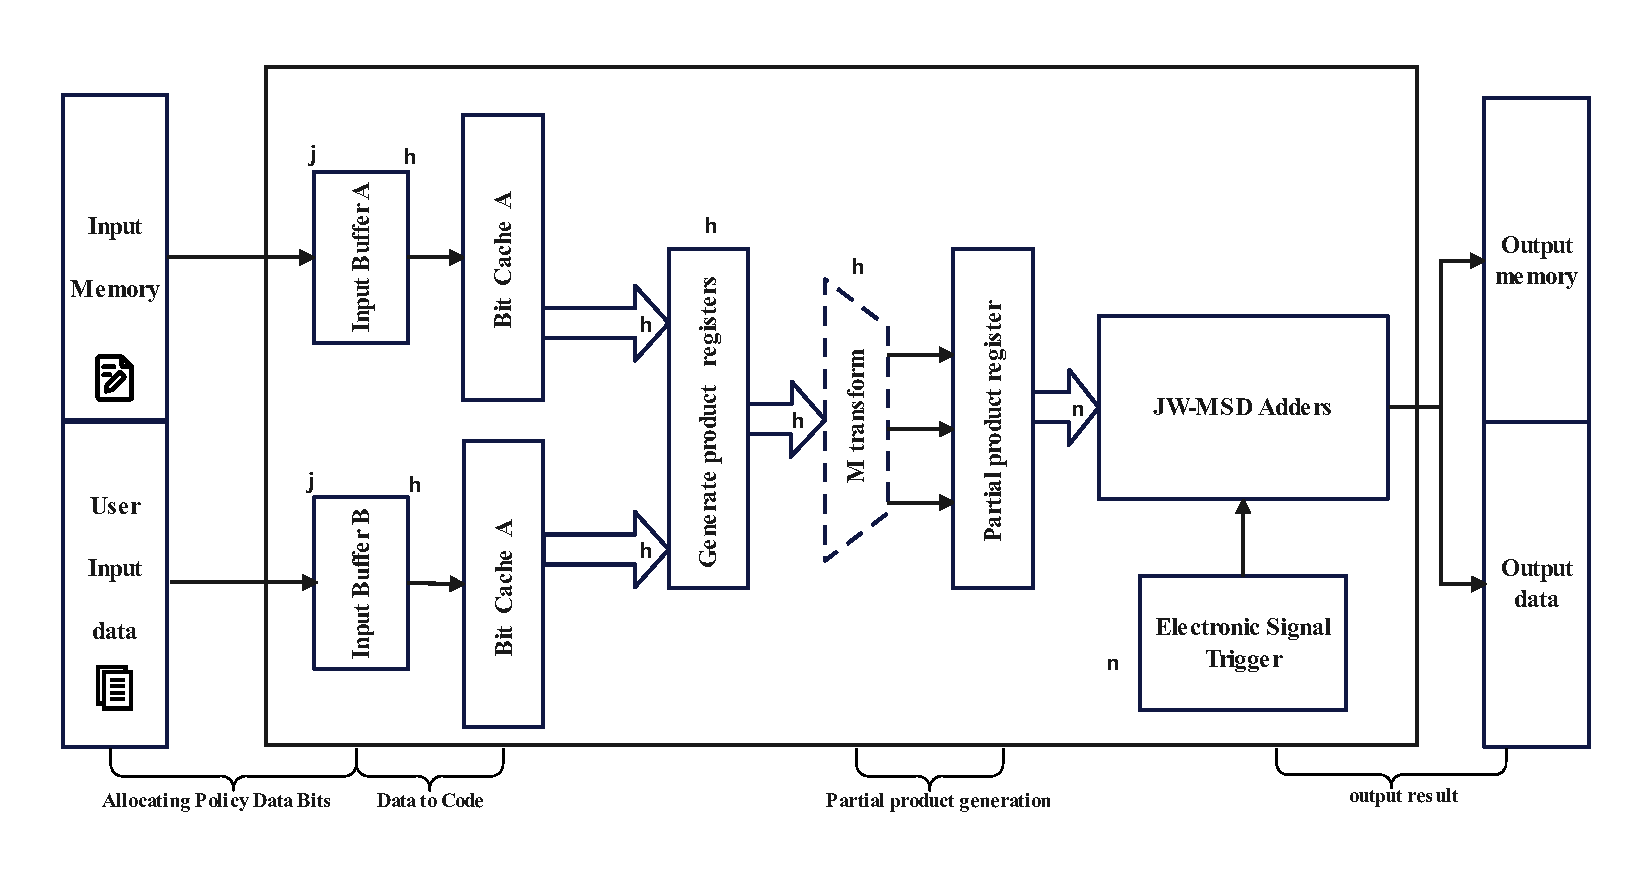
\includegraphics[scale=0.5]{./images/1.pdf}
   % \captionsetup{justification=centering} 
    \caption{RFLMR  structure diagram}
    \label{fig1}
\end{figure}


To overcome these challenges, reconfigurable multi-valued logic electronic processors have emerged, drawing on the research theories of ternary optical computers \cite{ref1,ref2,ref3,ref4,ref5,ref6,ref7,ref19}, particularly the structure and characteristics of the SD16 ternary optical processor\cite{ref21,ref22,ref23,ref24}. A patent filed by Professor Jin Yi and others in January 2019, titled “A Multi-Valued Logic Electronic Processor with Numerous Bits, Grouping Capability, and Reconfigurability, and Method,” laid the foundation for the development of such processors\cite{ref8}.In 2021, Wang et al. implemented a reconfigurable four-valued logic processor on an FPGA and tested it with various four-valued logic operations\cite{ref9,ref10,ref11,ref12}, verifying the effectiveness and reconfigurability of the processor architecture and circuits. Based on the theory of reduced-value design\cite{ref13,ref14}, the reconfigurable multi-valued logic electronic processor can dynamically determine the current computational function of the processor by inputting different reconfiguration instructions, meaning that the computational function of each processor bit can be reconfigured independently. By combining these bits, a multi-valued logic processor structure with numerous bits and its reconfigurable circuits can be constructed. This paper utilizes multiple computational bits of the reconfigurable four-valued logic processor to build a JW-MSD adder. The characteristic of this adder is that there is no carry relationship between data bits, allowing all data bit addition operations to be completed synchronously without considering carry dependencies between bits. On this basis, we designed and implemented a reconfigurable quaternary logic multiplication routine, as shown in Figure \ref{fig1}. During the reconfigurable quaternary logic multiplication process, input and output memory serve as crucial channels for data interaction between the user and the system. Input data is stored in the Input Memory and converted into MSD numbers through a bit allocation strategy. Then, auxiliary data is generated from the input MSD numbers via Bit Cache A and Bit Cache B, followed by an M Transform to obtain partial products. Finally, the electronic signal trigger activates the JW-MSD adder to perform accumulation operations, thus completing the multiplication routine calculation. The proposed reconfigurable quaternary logic multiplication routine provides a novel approach for ternary logic operations, laying a solid foundation for designing more complex ternary logic computing systems in the future.

%%%%%%%%%%%%%%%%%%%%%%%%%%%%%%%%%%%%%%%%%%
\section{MSD Digital System}
The Modified Signed-Digit (MSD) numeral system represents a pivotal innovation in digital computation\cite{ref15,ref16,ref17,ref18}
,primarily due to its ability to perform non-carry addition, thereby significantly enhancing computational efficiency. The concept of MSD can be traced back to the 1960s when computer scientists actively sought new methods to improve computational speed and performance. Traditional binary numeral systems faced substantial challenges with carry mechanisms when processing large volumes of data. To address this core issue, the concept of MSD was introduced and gradually evolved into an effective solution.The introduction and development of MSD have profoundly impacted modern computer science. Firstly, it cleverly circumvents the carry problem inherent in traditional binary systems, leading to a leap in computational speed. Secondly, the application of MSD in optical computing has driven innovation and progress in optical computing technology. More importantly, the non-carry characteristic of MSD demonstrates significant advantages in large-scale parallel computing scenarios, providing robust support for high-performance computing.Therefore, MSD not only enriches the theoretical methods of numerical representation but also promotes optimising and upgrading computer hardware and software systems in practical applications, laying a solid foundation for efficient computing in the era of big data.
\subsection{MSD Number}
Traditional electronic computers use binary (0 and 1) for computation, where any decimal number has a unique representation. However, the ternary optical computer (TOC) adopts the MSD number system, which represents a signed ternary binary number. The same decimal number can have multiple representations, providing a theoretical basis for carry-free addition. This system was first proposed by A. Avizienis et al. in 1961 and introduced into the field of optical computing by Drake et al. in 1986. The symbol set for this system is {u, 0, 1}, where you represent the value -1. Any decimal number D can be represented using the MSD number system, with its expression shown in formula  \ref{eq1}:
\begin{equation}
A = \sum_{i} a_i \times 2^i
\label{eq1}
\end{equation}
In the above formula, the value of $a_i$ is \{u, 0, 1\}, where i is a natural number, and $2^i$ indicates that the number is still a binary number.

\subsection{MSD Number Characteristics}
Due to redundant notation, MSD numbers have the following characteristics compared to regular binary number representations.
\begin{enumerate}
    \item In addition to the data 0 value, any value has an infinite number of MSD number expressions, such as:
    $[-32]_{10}=[u00000]_M=[u100000],[5.5]_{10}=[101.1]_M=[10uu.1]_M$
    \item The MSD number of a value is inverted bit by bit (0 is unchanged, and one and u are converted to each other) to obtain the MSD number of the opposite of the value:
    $[-15]_{10}=[uuuu]_M=-[1111]_M,[-7]_{10}=[uuu]_M=-[111]_M$
\end{enumerate}
\subsection{MSD Addition}
MSD addition differs from conventional binary addition in that it is accomplished through four transformations: \textit{T},\textit{ W}, \textit{T’}, and \textit{W’} (as shown in Table \ref{tab1}). These four transformations are ternary logic operations. Due to the redundancy of MSD, the corresponding addition can be completed in just three clock cycles, regardless of the number of bits in the addends\cite{ref20}. Suppose there are MSD numbers $A = \sum a_i \times 2^i$ (i=0,1,…,n-1), and MSD number B = $\sum b_j \times 2^j$(j=0,1,…,m-1).

The symbol sets for $a_i and b_j$ are both {u, 0, 1}, where n and m are positive integers, and i and j are natural numbers,(0 $\leq i \leq n-1), (0 \leq j \leq m-1)$. The MSD addition process is as follows:

\begin{enumerate}[label={\arabic*).}]
\item  Perform\textit{ T} and \textit{W} operations bitwise on the inputs \textit{A} and \textit{B}. (The result of the T operation is padded with 0 on the lower bit, and the result of the W operation is padded with 0 on the higher bit).
\item Perform \textit{T’} and \textit{W’} operations bitwise on the results of the first step. (The result of the \textit{T’} operation is padded with 0 on the lower bit, and the \textit{W’} operation is padded with 0 on the higher bit).
\item  Perform $T_2$ operations bitwise on the results of the second step to obtain the sum of \textit{A} and \textit{B} finally.
\end{enumerate}

\begin{table}[H]
\caption{\textit{T}, \textit{W}, \textit{T'} and \textit{W'}, $T_2$ transformations}
\label{tab1}
\centering
\begin{tabular}{*{20}{c}}
  \toprule
  &&$T$& & &&$W$& & & &$T'$ &  &&&$W'$ & & & & $T_2$ \\
\cmidrule(l{5pt}){1-20}
  \multirow{2}{*}{b} & \multicolumn{3}{c}{a(t')} &\multirow{2}{*}{b}& \multicolumn{3}{c}{a(t)}  &\multirow{2}{*}{b}& \multicolumn{3}{c}{w(t')} &\multirow{2}{*}{b}& \multicolumn{3}{c}{w(t)}&\multirow{2}{*}{b}& \multicolumn{3}{c}{a(t')} \\
  \cmidrule(lr){2-4}\cmidrule(lr){6-8}\cmidrule(lr){10-12}\cmidrule(lr){14-16}\cmidrule(lr){18-20}
  & u & 0 & 1 & & u & 0 & 1 & & u & 0 & 1 & & u & 0 & 1 & & u & 0 & 1 \\
  \midrule
   u& u & u & 0 & u & 0 & 1 & 0 & u & u & 0 & 0 & u & 0 & u & 0 & u & u & u & 0\\
   0& u & 0 & 1 & 0 & 1 & 0 & u & 0 & 0 & 0 & 0 & 0 & u & 0 & 1 & 0 & u & 0 & 1\\
   1& 0 & 1 & 1 & 1 & 0 & u & 0 & 1 & 0 & 0 & 1 & 1 & 0 & 1 & 0 & 1 & 0 & 1 & 1\\
  \bottomrule
\end{tabular}
% \captionsetup{justification=centering}

\end{table}
The MSD number system's unique redundancy property enables the feasibility of parallel addition operations. This characteristic stems from the inherent attribute of the MSD number representation, where the computation of each digit does not need to wait for a carry signal, thereby breaking the limitation of sequential digit computation in traditional serial adders. Specifically, during the MSD addition process, the result of each digit can be generated independently, unaffected by the operations of other digits. This provides the theoretical foundation for achieving fully parallel logic transformations within a single cycle. Therefore, the parallel addition mechanism under the MSD architecture not only enhances computation speed but also optimizes the utilization efficiency of hardware resources, demonstrating potential advantages in the field of high-performance computing.
%%%%%%%%%%%%%%%%%%%%%%%%%%%%%%%%%%%%%%%%%%
\section{Implementation Mechanism of the RFLMR }
\subsection{Working Principle of the RFLEP}
The circuit structure of the  RFLEP is shown in Figure \ref{fig2}. This processor contains multiple processor bits (m bits). In the figure, label \circled{1} represents the 0th bit of the processor, with the output signal being $C_0$(n value); label \circled{2} represents the (m-1)th bit of the processor, with the output signal being $C_{m-1}$(n value). The structure of each processor bit is identical. As shown in \circled{1}, each processor bit includes n column operators (such as \circled{3} and \circled{4}) and a potential combiner, as illustrated in Figure \ref{fig2}. Among them, \circled{3} is the 0th column operator of the 0th operator bit, with the output being ${Co}^0$(n value); \circled{4} is the (n-1)th column operator of the 0th operator bit, with the output being ${C_o}^{n-l}$(n value). The structure of the column operators in each processor bit is the same. As shown in\circled{3}, each column operator includes a high-impedance gate \circled{5}, a level multiplexer\circled{6}, an A signal selector \circled{7}, a work enabler \circled{8}, a reconfiguration latch\circled{9}, and a reconfiguration circuit \circled{10}.
\begin{figure}[H]
%\centering
    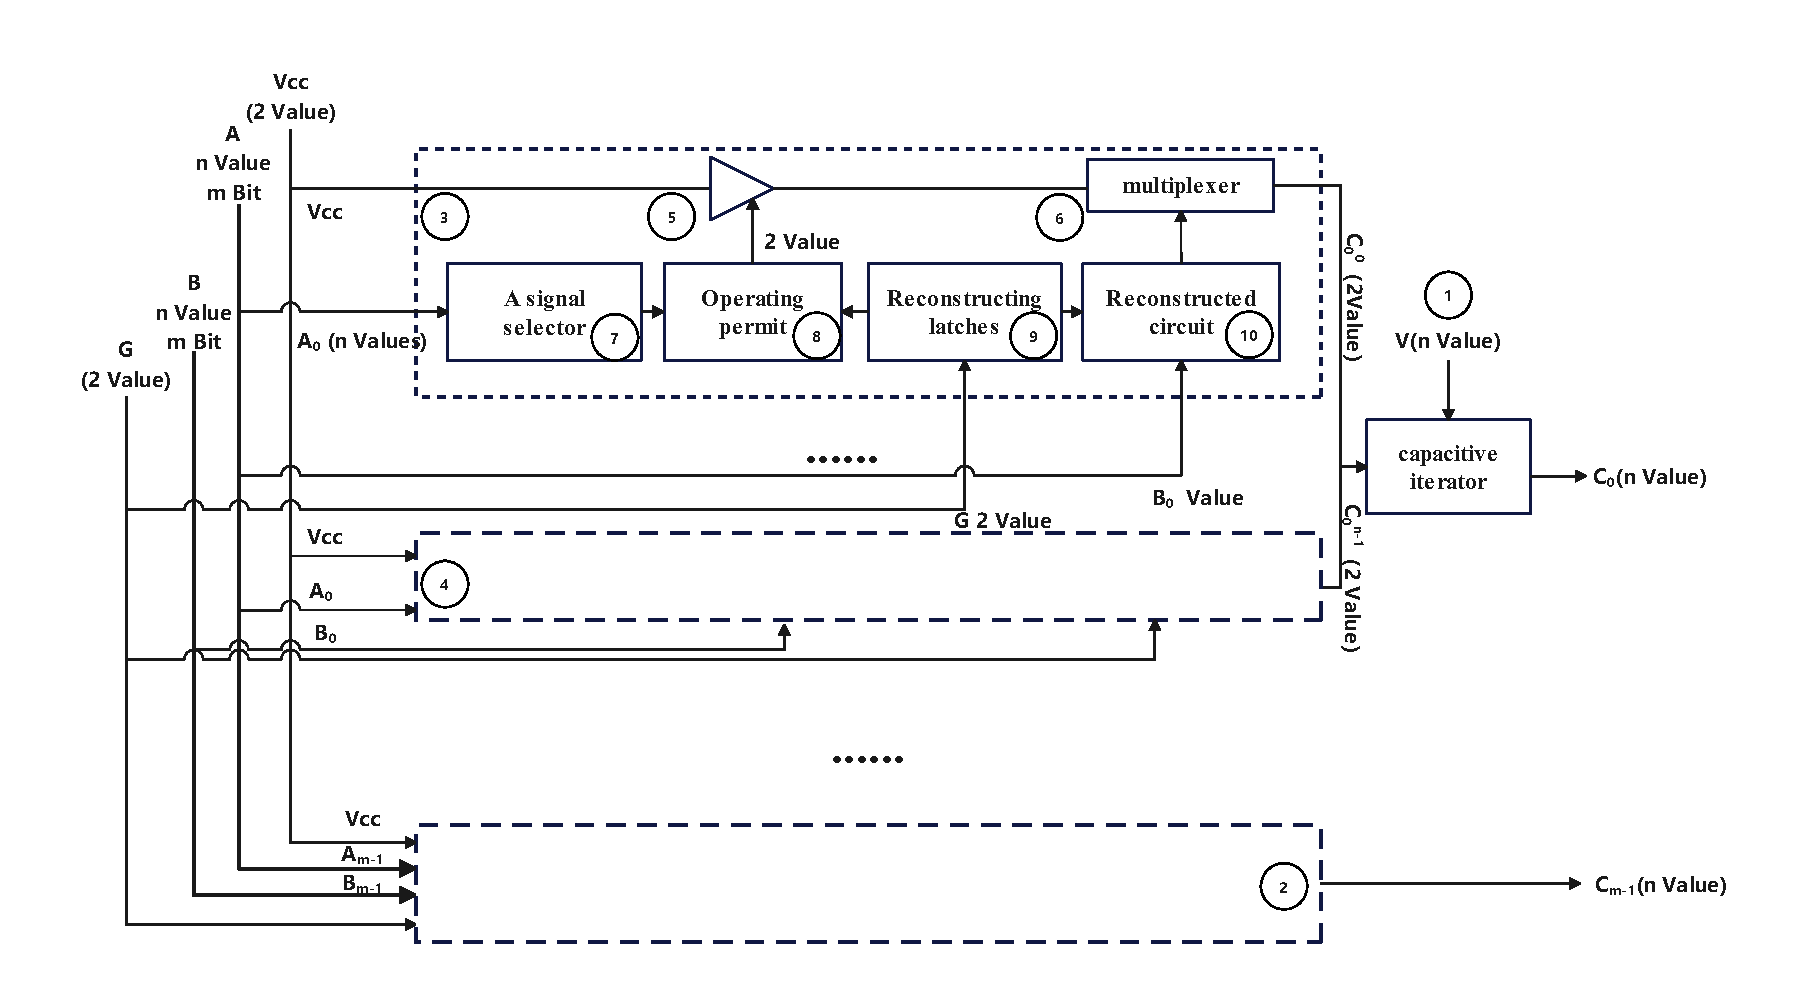
\includegraphics[scale=0.45]{./images/2.pdf}
  %  \captionsetup{justification=centering} 
    \caption{Schematic diagram of RMLEP architecture}
    \label{fig2}
\end{figure}
In Figure \ref{fig2}, the RFLEP writes reconfiguration instructions into the reconfiguration latch via the G signal line. These reconfiguration instructions determine the operational function of each column operator, enabling one of the n(n×n) types of logical operations. The reconfiguration circuit has p branches, and since each n-value signal requires p binary signals to represent it, p is equal to the square root of n rounded up. Each branch of the reconfiguration circuit selects and simply transforms the i-th bit of the data B input to the branch based on the signal state of the branch control end and sends the selection and transformation result to the input end of the output generator through the output end of the branch. The input end of the output generator also has p input lines. The potential combiner of the i-th bit of the constructed operator combines the output signals of all column operators of that operator bit to form the physical output signal of that operator bit. Since any value of the i-th bit of data A meets the selection requirements of the A signal selector of a column operator, the operator bit can perform logical operations on any value of the i-th bit of data A and the i-th bit of data B.Therefore, by sending different reconfiguration instructions to the reconfiguration circuit of the general structure of the RFLEP, the current logical operation function of the processor can be dynamically configured, forming specific logical operators and achieving reconfigurable logical operation functions for each processor.
\subsection{Reconfigurable Four-Valued Logic JW-MSD Adder Principle}
Based on in-depth research on MSD  addition theory, our research team has designed and implemented an innovative parallel adder circuit architecture—the JW-MSD adder. The uniqueness of this adder lies in its specially customized ternary logic operation unit, which closely aligns with the logical requirements of the MSD addition algorithm. Streamlining the number of logic gates significantly enhances the efficiency and speed of dedicated addition operations. The ternary logic operator plays a crucial role in the core design of the JW-MSD parallel adder. Compared to traditional binary adders, which often require complex circuit layouts to handle carry propagation, the MSD adder leverages its ternary logic (u, 0, 1) characteristics to avoid the complexity of carry operations, thereby significantly accelerating computation speed and enhancing operational efficiency. Building on this, the JW-MSD adder further optimizes the design of the ternary logic operator, greatly simplifying the overall circuit structure and effectively reducing the number of logic gates used, achieving a dual optimization of performance and cost-effectiveness. Figure \ref{fig3} shows the circuit schematic of our developed specialized JW-MSD parallel adder, providing readers with a clear visual reference to facilitate a deeper understanding of the working mechanism of the JW-MSD adder.
\begin{figure}[H]
%\centering
    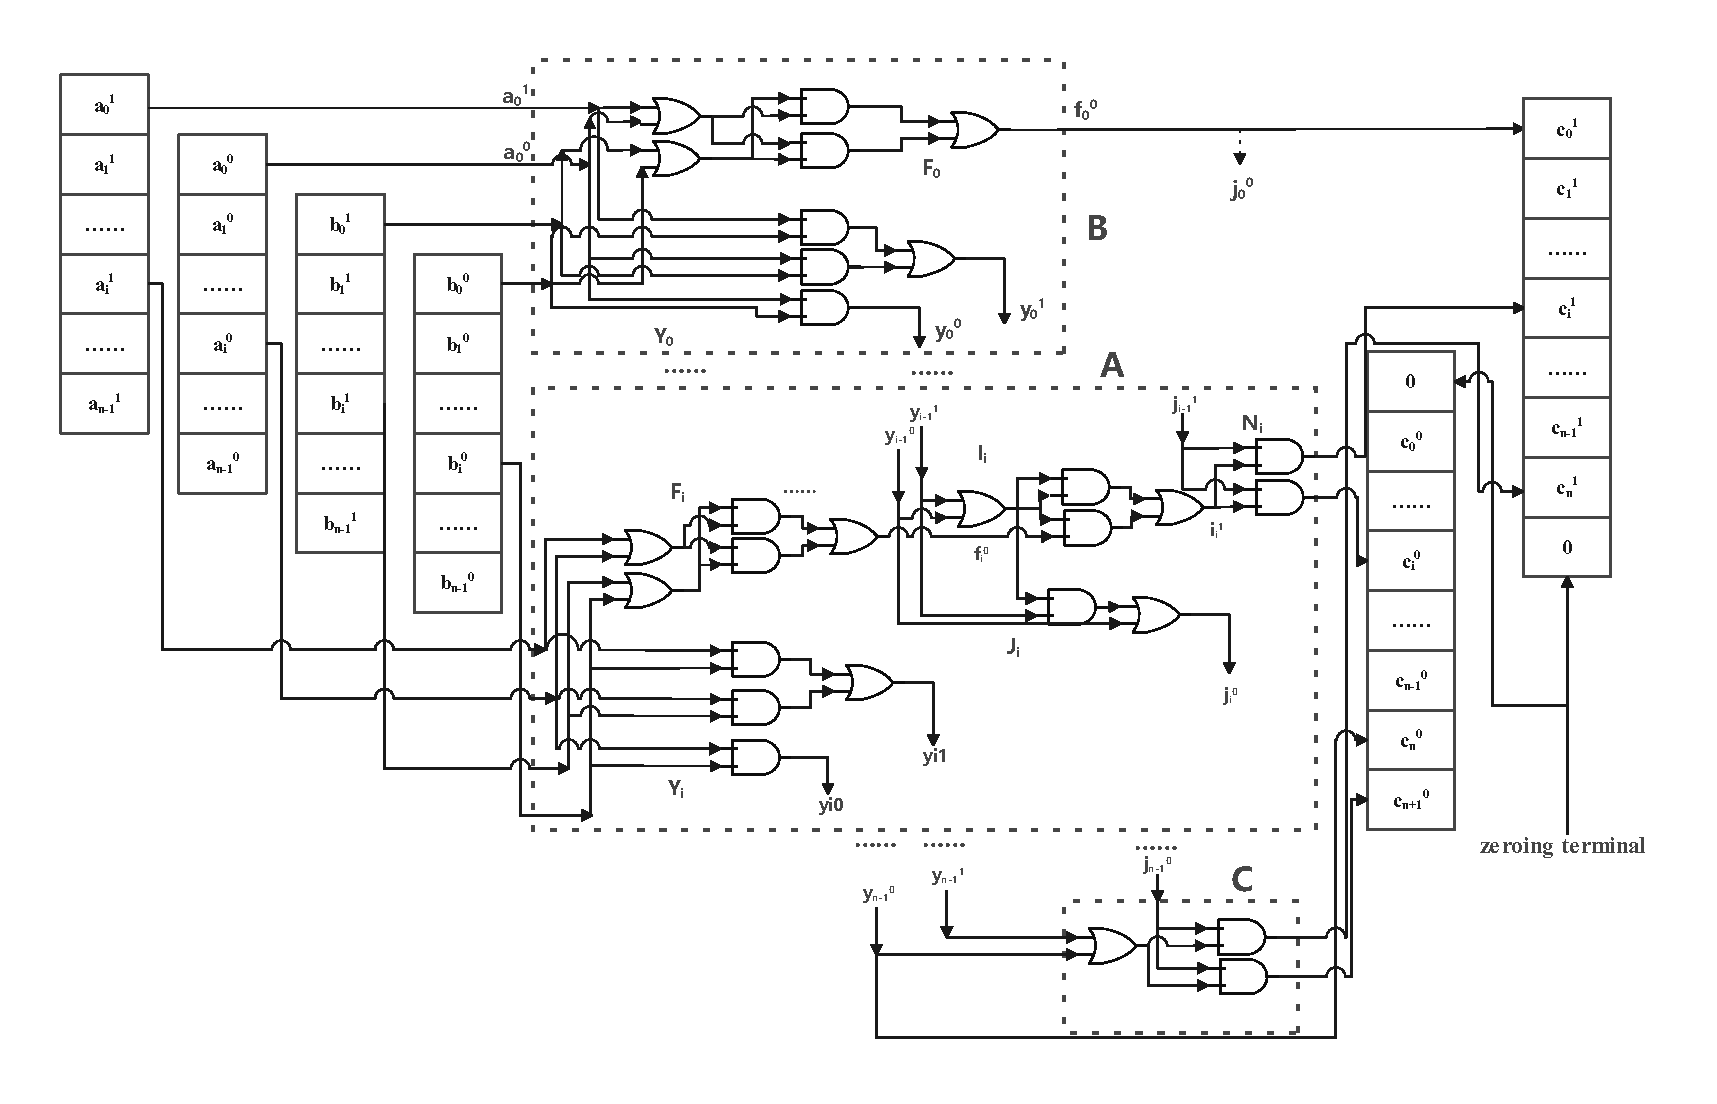
\includegraphics[scale=0.45]{./images/3.pdf}
   % \captionsetup{justification=centering} 
    \caption{JW-MSD adder structure schematic diagram}
    \label{fig3}
\end{figure}
The n-bit specialized JW-MSD parallel adder consists of five ternary logic operators, namely the Y operator, F operator, J operator, I operator, and N operator, as shown in Table \ref{tab2}. They use three two-bit binary symbols “00”, “01”, and “10” to represent the MSD numbers “0”, “u”, and “1”. This n-bit specialized JW-MSD parallel adder is composed of three operation modules, as well as input and output registers. The three operation modules are the\textit{ A} operation module, \textit{B} operation module, and \textit{C} operation module. For this n-bit specialized JW-MSD parallel adder, the input operands of the adder are represented by $a_{n-1} a_{n-2}...a_1 a_0$ and $b_{n-1} b_{n-2}...b_1 b_0$, and the output is represented by $c_{n-1} c_{n-2}...c_1 c_0$. Each bit is represented by two binary bits, so ${a_i}^0$ represents the low bit input of the i-th bit, ${a_i}^1$ represents the high bit input of the i-th bit; ${b_i}^0$ represents the low bit input of the i-th bit, ${b_i}^1$1 represents the high bit input of the i-th bit; ${c_i}^0$ represents the low bit output of the i-th bit, and ${c_i}^1$represents the high bit output of the i-th bit. The operation cycle of this adder can be divided into three steps:

\begin{enumerate}[label={\arabic*).}]
\item  First, the n-bit input operands a and b are written into the high and low bit registers of input register a and the high and low bit registers of input register b, respectively, while the low bit signal $c_0^0$ of the 0th bit and the high bit signal $c_{n+1}^1$ of the (n+1)th bit of the output register is cleared to 0.
\item Second, after the calculations of each operation module, the final output result is obtained. This step involves a delay of 6 layers of binary logic gates, and the calculation result is finally stored in the output register.
\item  Third, data is read from the output register to construct the n-bit specialized JW-MSD parallel adder, which requires 7×n+5 two-input OR gates, $10 \times n+7$ two-input AND gates, and $9 \times n+6$ single-input NOT gates. Therefore, the n-bit specialized JW-MSD parallel adder will use fewer logic gate devices.
\end{enumerate}

\begin{table}[H]
\caption{Five ternary logic operators of JW-MSD parallel adder}
\label{tab2}
\centering
\resizebox{1\textwidth}{!}{%
\begin{tabular}{|c|c|c|c|c|c|c|c|c|c|c|c|c|c|c|c|c|c|c|c|}
\hline
\multicolumn{4}{|c|}{Y operator} & \multicolumn{4}{c|}{F operator} & \multicolumn{3}{c|}{J operator} & \multicolumn{3}{c|}{I operator} & \multicolumn{3}{c|}{N operator} \\ \hline
\diagbox{$a_i$}{$b_i$} & 00 & 01 & 10 & \diagbox{$a_i$}{$b_i$} & 00 & 01 & 10 & \diagbox{$y_i$}{$f_i$} & 00 & 01 & \diagbox{$y_i$}{$f_i$} & 00 & 01 & \diagbox{$j_i$}{$i_i$} & 00 & 10 \\ \hline
00 & 00 & 00 & 10 & 00 & 00 & 01 & 01 & 00 & 00 & 01 & 00 & 00 & 10 & 00 & 00 & 10 \\ \hline
01 & 00 & 01 & 00 & 01 & 01 & 00 & 00 & 01 & 01 & 01 & 01 & 10 & 00 & 01 & 01 & 00 \\ \hline
10 & 10 & 00 & 10 & 10 & 01 & 00 & 00 & 10 & 00 & 00 & 10 & 10 & 00 &     &    &    \\ \hline
\end{tabular}
}
% \captionsetup{justification=centering} 

\end{table}

%%%%%%%%%%%%%%%%%%%%%%%%%%%%%%%%%%%%%%%%%%
\subsection{RFLMR Implementation}
\subsubsection{Partial Product Generation and Summation Key Techniques}
For implementing the MSD  multiplication routine, the main core points include the generation of partial products and the summation of partial products. This paper delves into the implementation strategies for these two aspects. Suppose the multiplicand A has n bits, represented as $A=a_{n-1} a_{n-2}...a_1 a_0$, with its MSD expression being $A=\sum a_i \times 2^i$, where i ranges from 0 to n-1. Similarly, the multiplier B has m bits, represented as $B=b_{m-1} b_{m-2}...b_1 b_0$, with its MSD expression being $B=\sum b_j \times 2^j$, where j ranges from 0 to m-1. The symbols $a_i$ and $b_j$ are both from the set {u, 0, 1}, where n and m are positive integers, and i and j are natural numbers, satisfying $0 \leq i \leq n-1,0 \leq j \leq m-1$. Thus, the MSD multiplication routine can be expressed by formula \ref{eq2}.
\begin{equation}
C=A \times B=A \times \sum b_j \times 2^j = \sum A \times b_j \times 2^j=\sum S_j \times 2^j=\sum P_j
\label{eq2}
\end{equation}

Based on the above formula \ref{eq2}, the MSD multiplication process is as follows:
\begin{enumerate}[label={\arabic*).}]
\item In $C=A \times B$,\textit{ A} is the multiplicand, and \textit{B} is the multiplier. B is generated as $B=\sum b_j       
      \times 2^j $. Each bit $b_j$ of B\textit{} generates auxiliary data with p bits of $b_j$ values. $b_j$ and \textit{A }undergo \textit{M} transformation bitwise to obtain j partial products $S_1, S_2,…, S_j$, the M transformation table is shown in Table \ref{tab3}.
\item  Each partial product $S_j$ is shifted left by j - 1 bits, j - 1 zeros are appended to each          $S_j$, resulting in j sum terms $P_1, P_2,…, P_j$.
\item The j sum terms $P_1, P_2,…, P_j$ are summed using an MSD adder, and the accumulated result   
      is the product \textit{C}.
\end{enumerate}


\begin{table}[H]
\caption{\textit{M} transformation}
\label{tab3}
%\centering
\resizebox{0.4\textwidth}{!}{%
\begin{tabular}{cccccccc}
  \toprule
  & & & \textit{M} & & & & \\
  \cmidrule(lr){1-8}
  \multirow{2}{*}{b}   & &  & &a && \\
  \cmidrule(lr){3-7}
  && u & & 0 & & 1 &  \\
  \midrule
  u && 1 & & 0 & & u &  \\
  0 && 0 & & 0 & & 0 &  \\
  1 && u & & 0 & & 1 &  \\
  \bottomrule
\end{tabular}%
}
\captionsetup{justification=centering} 
\end{table}

\subsubsection{RFLMR Design}
The RFLMR is implemented through programming on the Alinx7020, as shown in Figure 4. It consists of six operators and 199 processor bits. Since electronic transistors can only represent binary, we use two binary bits to represent MSD numbers. Specifically, the three MSD states (such as u, 0, 1) can be represented by binary 00, 01, and 10, respectively. In this representation method, each bit combination is realized through the on-and-off states of electronic transistors. This design not only maintains the characteristics of ternary logic but is also compatible with the binary representation of electronic transistors, making it possible to implement the RFLMR on the Alinx7020 through the Processor System (PS) and Programmable Logic (PL) parts. The design of the multiplication routine is mainly divided into four parts:

\begin{enumerate}[label={\arabic*).}]
\item  \textbf{MSD Number Conversion}: First, the input binary number must be converted into an MSD number representation. This step is crucial as it lays the foundation for subsequent partial product generation and addition operations. Our design implements MSD number conversion through the MSD\_transform function on the PS side. The core objective of the MSD\_transform function is to convert a given decimal number ( \textit{D} ) into its corresponding MSD representation. Assuming we have a decimal number ( \textit{D} ), we first convert its absolute value ( \textit{|D|} ) into a binary representation. If ( 0 < \textit{D} ), the resulting binary number is inverted; otherwise, it remains unchanged. Then, the obtained binary number is converted into the corresponding MSD number, where 00, 01, 10, etc., represent different digits.
\item \textbf{Partial Product Generation}: During partial product generation, the multiplier ( \textit{B} ) first generates auxiliary data for each bit, which is stored in registers through the generate\_auxiliary\_data function. Then, the auxiliary data corresponding to each bit ( $b_j$ ) in the register is sent to the arithmetic unit ( \textit{S} ) along with each bit of the multiplicand ( \textit{A }) for computation. Specifically, for each bit ( $b_j$ ), an M-logic operation with the multiplicand ( \textit{A} ) is performed to generate the partial product ( $S_j$ ). To improve computational efficiency, M-transformation uses parallel computing technology. By implementing parallel operations in hardware, multiple partial products can be computed simultaneously, reducing computation time. The computed partial products ( $S_j$ ) are stored in registers for subsequent shifting and summation operations.
\item  \textbf{Partial Product Shifting}: After generating the partial products, each partial product needs to be shifted for subsequent summation calculations. Each partial product ( $S_j$ ) needs to be left-shifted by ( \textit{j-1} ) positions, with ( \textit{j-1} ) zeros appended to the end of each ( $S_j$ ) through the shift\_operation function, resulting in partial products ($P_1, P_2, \ldots, P_j$ ). This operation is implemented using hardware shift registers to ensure the efficiency of the shifting operation.
\item \textbf{Partial Product Summation}: Partial product summation is the crucial step in generating the final product (\textit{ C }), achieved through the JW-MSD adder, which uses ternary logic to sum different partial products quickly. On the PL side, partial products are sent to the JW-MSD adder for computation through the MSD\_33\_mWriteReg function. Given the abundant hardware logic units in the Alinx7020, multiple JW-MSD adders can be configured on the PL side. Due to the redundancy characteristics of MSD numbers (see 2.3 MSD Number Characteristics), the summation of partial products ( $P_1, P_2, \ldots, P_j$ ) adopts parallel computing methods. Rapid accumulation is achieved by cascading and pipelining multiple levels of MSD adders, resulting in the final MSD product. This result is then transmitted to the platform for display and further processing. The entire process is highly parallel and flexible, enabling efficient digital computation. 
\end{enumerate}


\subsubsection{Pipelined Design of RFLMR}
In this study, we delve into the multiplication operation ( $A \times B = C$ ), where ( \textit{A} ) and ( \textit{B} ) have ( \textit{m} ) and (\textit{ n} ) MSD digits respectively, satisfying ( \textit{0 < m < 33} ) and (\textit{ 0 < n < 33} ). For the multiplication routine processor architecture, we propose a novel and efficient computational method that combines M transformation with JW-MSD addition technology, where ( \textit{B} ) acts as the multiplier and ( \textit{A} ) as the multiplicand. This process involves ( \textit{n }) M transformations and their associated partial cumulative addition operations. We fully utilize the inherent redundancy of MSD numbers to optimize multiplication efficiency. Therefore, we introduce a multiplication routine based on reconfigurable four-valued logic and implement a pipeline design strategy to facilitate smooth and fast data processing. The core idea of the pipeline design is to break down complex operations into several independent stages, allowing each stage to process different data segments in parallel or sequentially. This architecture is particularly suitable for the Alinx7020 platform, where precise management of clock cycles and operation segmentation ensures the efficiency and accuracy of the data processing flow.
\begin{figure}[H]
%\centering
    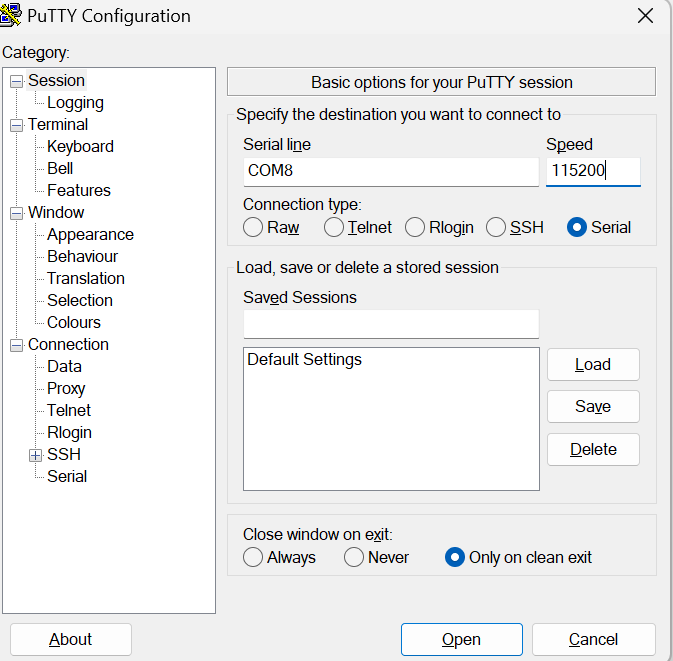
\includegraphics[scale=0.8]{./images/4.png}
   % \captionsetup{justification=centering} 
    \caption{Putty configuration diagram}
    \label{fig4}
\end{figure}
As shown in Figure \ref{fig5}, our pipeline design comprehensively covers the entire processing flow from input to output, illustrating the correspondence between the time sequence (measured in clock cycles) and each processing stage. Each periodic operation module—whether it is M transformation, T/W transformation, T’/W’ transformation, or T2 transformation—represents a specific processing step or operational unit in the pipeline. The parallel execution of these modules significantly enhances the overall processing speed.
\begin{figure}[H]
   % \centering
    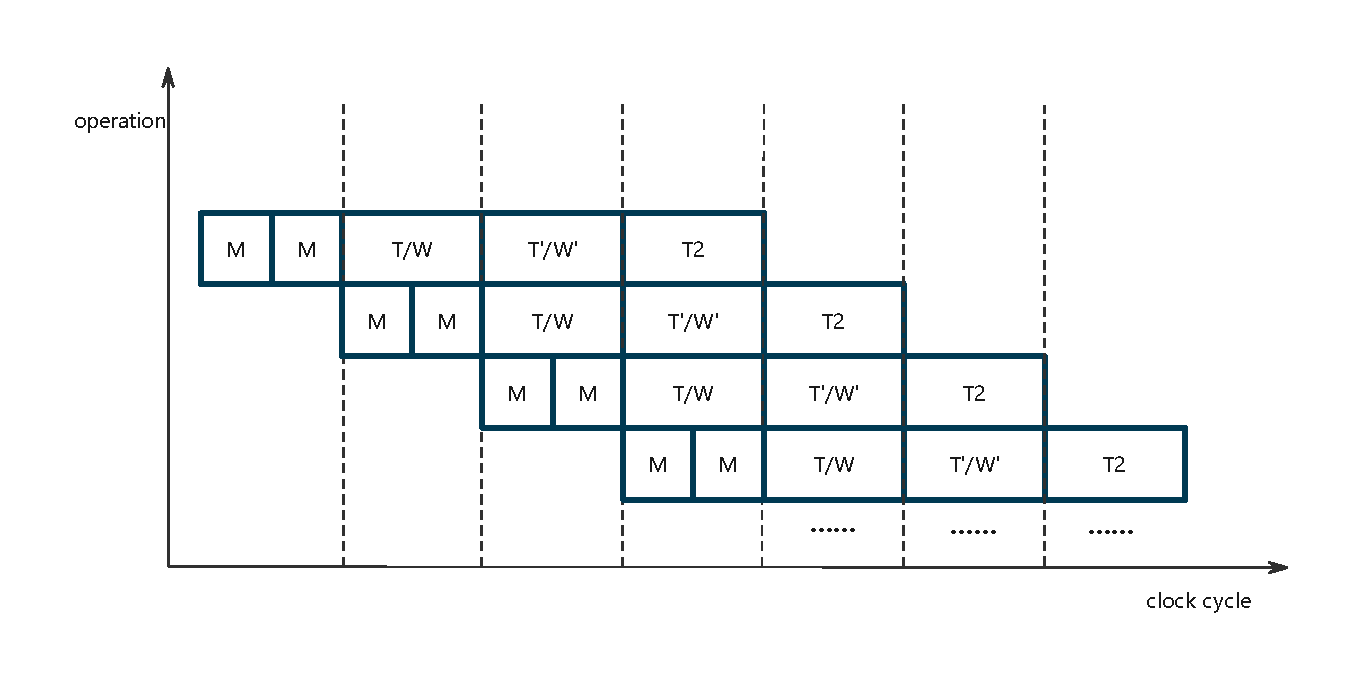
\includegraphics[scale=0.6]{./images/5.pdf}
 %   \captionsetup{justification=centering} 
    \caption{RFLMR pipeline diagrams}
    \label{fig5}
\end{figure}
%%%%%%%%%%%%%%%%%%%%%%%%%%%%%%%%%%%%%%%%%%
\section{Efficient Experiments with RFLMR}
\subsection{Experimental Preparation}
\subsubsection{Experimental Equipment}
In this experiment, we selected the Zynq7000 series chips from Xilinx as the core components. Specifically, we used the Alinx7020 core development board equipped with the XC7Z020-2CLG400I chip. This chip is renowned for its excellent pin compatibility and the 400-pin FBGA packaging technology it employs, ensuring design flexibility and efficiency. The unique feature of the Zynq7000 chip is its integration of the Processor System (PS) and Programmable Logic (PL) cores, achieving a perfect blend of hardware and software. The PS part on the Alinx7020 core board provides wealthy external interfaces and devices, greatly facilitating user operations and function verification processes.Meanwhile, each IO interface on the PL side is designed and routed to 2.54mm connectors on the board edge, offering users unlimited expansion possibilities to meet diverse needs from prototype design to product development. Notably, the core board is equipped with a 7 x 2 JTAG connector, allowing users to easily download and debug programs on the core board using Xilinx’s dedicated USB Cable downloader, significantly simplifying the development process. Figure \ref{fig6} vividly illustrates the overall architecture of the Alinx7020 system. With such a hardware layout and flexible interface configuration, the Alinx7020 provides stable and reliable hardware support, making it an ideal choice for exploring advanced computing technologies and implementing complex algorithms.
\begin{figure}[H]
   % \centering
    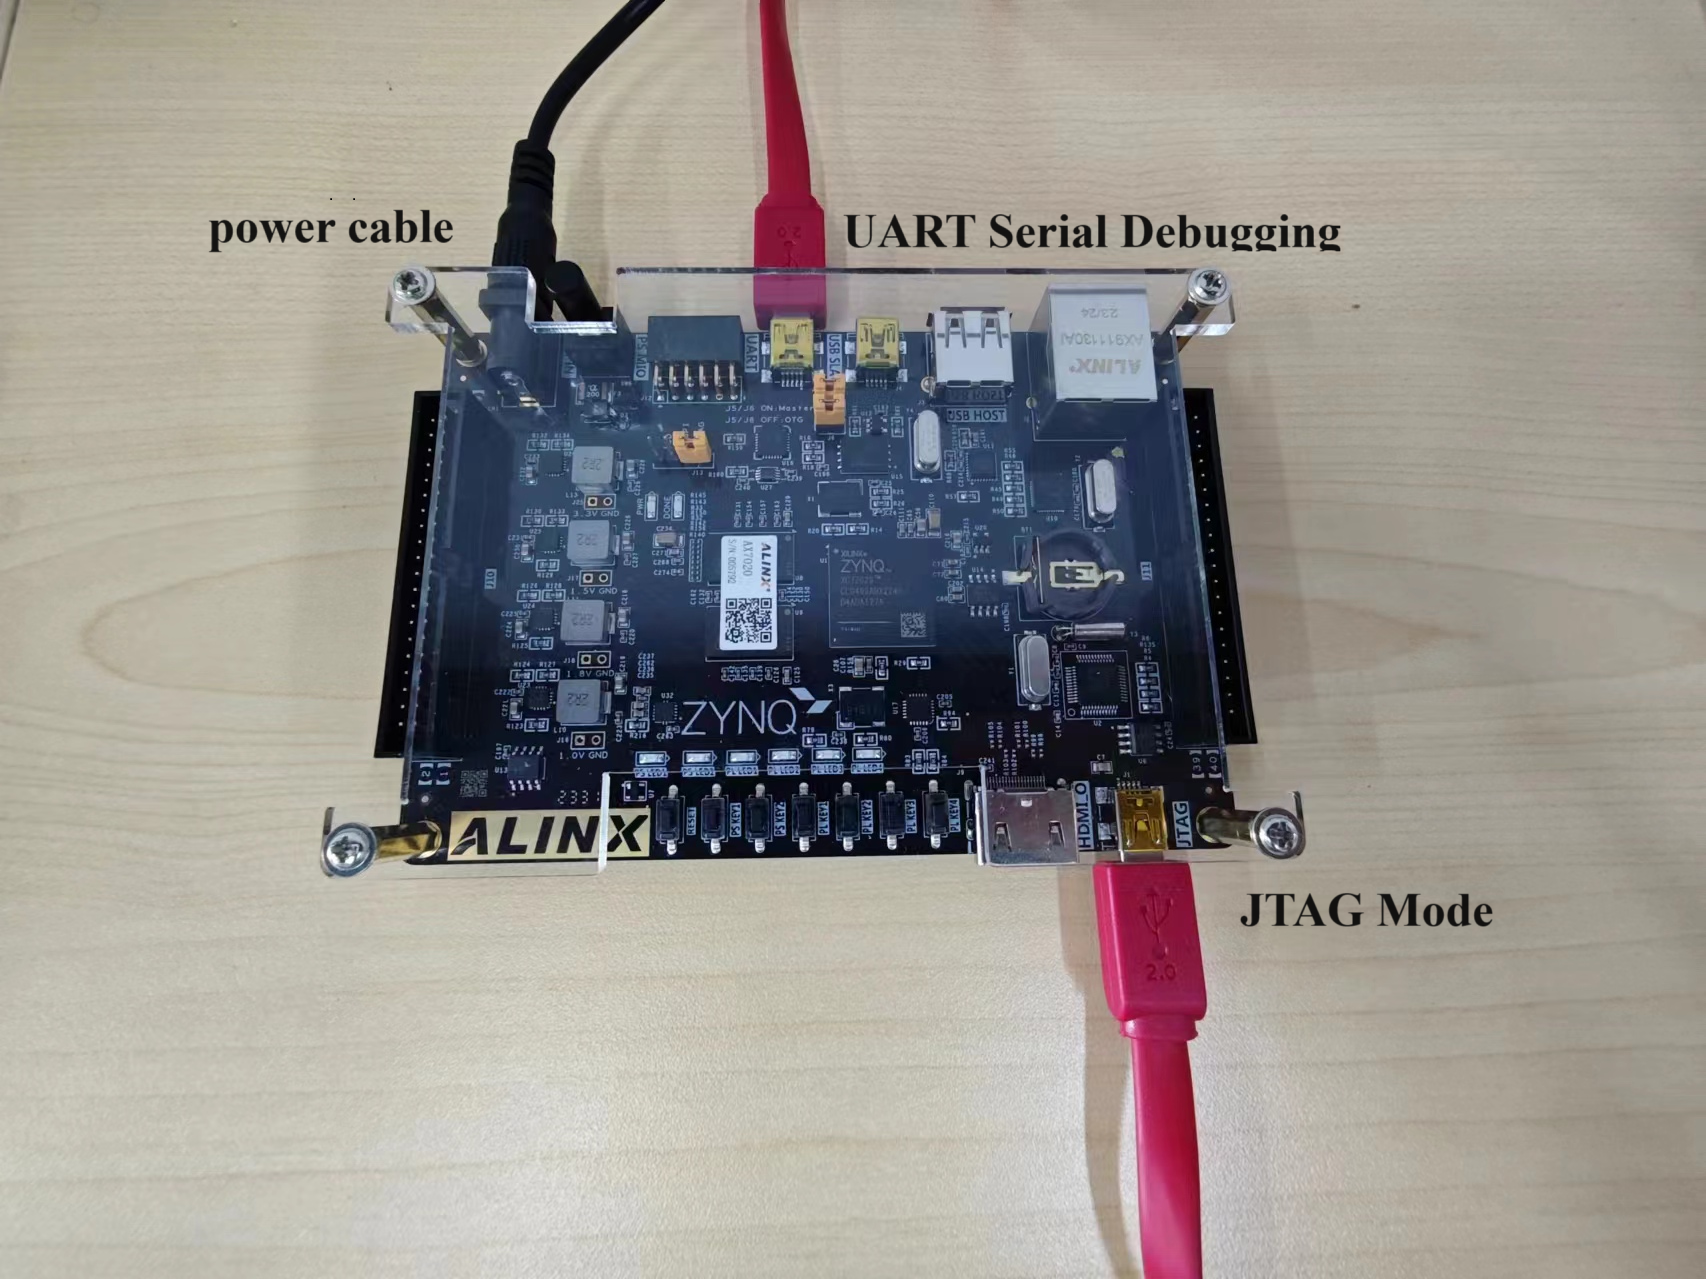
\includegraphics[scale=0.23]{./images/6.png}
   % \captionsetup{justification=centering} 
    \caption{ALinx7020 development board}
    \label{fig6}
\end{figure}
\subsubsection{Processor Bit Allocation Strategy for RFLMR}
On the Alinx7020 development board, we implemented the M transformation (S arithmetic unit) and JW-MSD adder in parallel within the Processor System (PS) and Programmable Logic (PL), as shown in Figure 7. Specifically, processor bits 0 to 32 are allocated for implementing the M transformation, while bits 33 to 198 are dedicated to constructing the JW-MSD adder. Each part of the design follows the bit allocation principles to ensure the efficient operation of the entire system. The layout of a 199-bit RFLMR processor is shown in Figure \ref{fig7}.
\begin{figure}[H]
 %%  \centering
    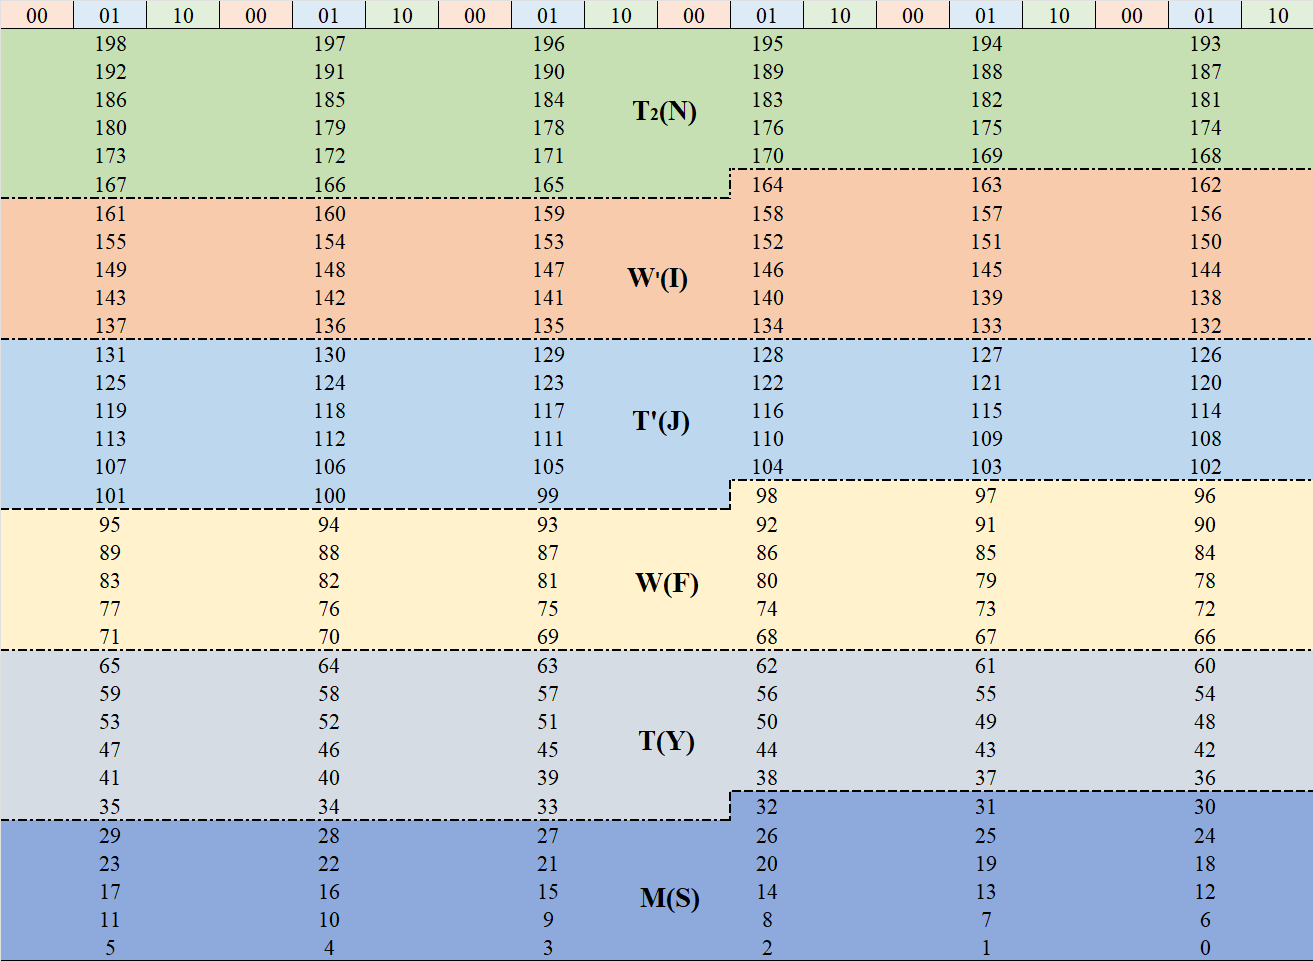
\includegraphics[scale=0.5]{./images/7.png}
  %  \captionsetup{justification=centering} 
    \caption{RFLMR processor bit allocation chart}
    \label{fig7}
\end{figure}
Specifically, for a 199-bit RFLMR processor, the allocation of processor bits is shown in Table \ref{tab4}.
\begin{table}[H]
    \caption{RFLMR processor bit allocation table}
    \label{tab4}
    \renewcommand{\arraystretch}{1.8}
%    \centering
    \scalebox{0.65}{
        \begin{tabular}{cccccc}
            \toprule
             \textit{M} & \textit{T} & \textit{W} & \textit{T'} & \textit{W'} & $T_2$ \\
            \midrule
             0\textasciitilde32(S operator) & 33\textasciitilde65(Y operator) & 66\textasciitilde98(F operator) & 99\textasciitilde131(J operator) & 132\textasciitilde164(I operator) & 165\textasciitilde198(N operator) \\
            \bottomrule
        \end{tabular}
    }
        \captionsetup{justification=centering} 
\end{table}
The rich hardware resources of the Alinx7020 development board provide a solid foundation for this multi-module parallel design. By executing each module in parallel without interference, we significantly improve the efficiency of the four-valued logic multiplication routine processor in handling complex computational tasks and greatly enhance its flexibility and reconfigurability. This design strategy allows for dynamic adjustment and optimization of the system based on different computational needs, demonstrating adaptability and high performance.
\subsection{Experimental Process of RFLMR}
\subsubsection{Test Cases}
To rigorously evaluate the accuracy of the RFLMR in handling arbitrary decimal values and ensure the correctness of outputs at each computational stage, this experiment designed a series of verification steps using registers as an essential aspect. We defined three core registers:
\begin{itemize}
    \item Register \textit{k} is used to store values converted from decimals to MSD.
    \item Register \textit{m }is responsible for recording partial products obtained after M transformation.
    \item Register \textit{s} are specifically used to retain the complete MSD calculation results.
\end{itemize}
Through this data management strategy, we can strictly monitor and ensure each computation's accuracy and the data's integrity.

Given that the processor bit width of the reconfigurable four-valued logic routine is set to 33 bits, its numerical expression range spans from ( $-3^{33}$ ) to ( $3^{33} - 1$ ), naturally constraining the bit width of the multiplicand and multiplier. To comprehensively examine the performance of this multiplication routine processor across a broad numerical domain, we conducted large-scale experiments, testing over ten thousand data samples. Although space limitations prevent a detailed discussion of each test, the selected cases are highly representative, and all test results consistently confirm the algorithm's effectiveness and accuracy. The experimental data (refer to Table \ref{tab5}) robustly demonstrate the computational capability and precision of the RFLMR processor across different numerical ranges.

\begin{table}[H]
    \renewcommand{\arraystretch}{1.2}
    \caption{ERLMR test cases}
    \label{tab5}
    \centering % 让标题居中
    \centering
    \label{tab5}
    \resizebox{\textwidth}{!}{% 调整表格大小
        \begin{tabular}{c c c c }
            \toprule
            Item &multiplication& Multiplier & Multiplicand  \\
            \midrule
            01 & $2 \times 3$ & $A(000000000000000000000000000000010)_M$ & $B(000000000000000000000000000000011)_M$ \\

            02 & $4 \times 5$ & $A(000000000000000000000000000000100)_M$ & $B(000000000000000000000000000000101)_M$  \\

            03 & $12 \times 15$  & $A(000000000000000000000000000001100)_M$ & $B(000000000000000000000000000001111)_M$ \\
       
            04 &  $-23 \times 34$  & $A(0000000000000000000000000000u0uuu)_M$ & $B(000000000000000000000000000100010)_M$ \\
           
            05 & $-67 \times -78$  & $A(00000000000000000000000000u0000uu)_M$ & $B(00000000000000000000000000u00uuu0)_M$ \\
          
            06 &  $123 \times 234$  & $A(000000000000000000000000001111011)_M$ & $B(000000000000000000000000011101010)_M$  \\
             
            07 &  $-345 \times 456$  & $A(000000000000000000000000u0u0uu00u)_M$ & $B(000000000000000000000000111001000)_M$ \\
          
            08 & $1234 \times 2345$ & $A(000000000000000000000010011010010)_M$ & $B(000000000000000000000100100101001)_M$ \\
      
            09 & $-3456 \times 4567$  & $A(000000000000000000000uu0uu0000000)_M$ & $B(000000000000000000001000111010111)_M$ \\
            \bottomrule
        \end{tabular}%
    }
% \captionsetup{justification=centering} 

\end{table}
\subsubsection{RFLMR Experimental Steps}
In constructing the RFLMR, we retained the input data interface on the PS side, connecting to the Alinx7020 core board via the Putty serial debugging tool to facilitate the input of test cases and the verification of results. The specific experimental implementation steps are as follows:
\begin{enumerate}[label={\arabic*).}]
\item \textbf{Hardware Connection and Configuration}: 
\begin{enumerate}[label=\protect\circled{\arabic*}] 
    \item Use Xilinx’s USB Cable to Download Files: As shown in Figure 4, connect one end of the USB Cable to the Alinx7020 board and the other to the host computer. Then, download the designed hardware configuration file to the Alinx7020 core board to ensure the core board correctly loads and runs our design. 
    \item Connect the JTAG Connector for Debugging: Download the required files to the Alinx7020 via the USB Cable, and then prepare the debugging program through the 7 x 2 JTAG connection. \end{enumerate}
\item \textbf{Software Environment Preparation}: 
    \begin{enumerate}[label=\protect\circled{\arabic*}] 
    \item Install and Configure the Putty Serial Debugging Tool: Download and install the Putty software on the debugging computer, ensuring the installation process is completed smoothly. 
    \item Set Serial Port Parameters: Open the Putty software and set the serial port parameters to a baud rate of 115200 and port number COM8. The detailed parameters and Putty graphical interface are shown in Figure 4 to match the communication requirements of the Alinx7020 core board. 
    \item Confirm Connection: In the Putty software, confirm that the serial port of the Alinx7020 core board is correctly recognized and connected, ensuring a smooth data transmission channel. 
    \end{enumerate}
\item \textbf{Input Test Cases}: 
    \begin{enumerate}[label=\protect\circled{\arabic*}] 
        \item Initialize Registers: Before inputting each test case, initialize registers k,  m, and s to 0 to ensure that the results of the previous operation do not affect the current calculation. 
        \item Input Test Cases: Sequentially input test cases 1 to 17 to the Alinx7020 core board through the Putty serial tool according to the designed order. Each test case includes two operands, and the multiplication routine processor will calculate and output the results based on the input. 
        \item Read Results: Read the output results of the multiplication routine processor for each test case. The results are shown in Table \ref{tab6}. 
        \end{enumerate}
\item \textbf{Display Experimental Results}: After inputting the test cases, observe the output of the Putty serial debugging tool and record the calculation results of each case. Compare the output results with the expected correct results. The calculation results are shown in Figure \ref{fig8}, verifying the performance and accuracy of the reconfigurable four-valued logic multiplier across different numerical ranges.
\begin{table}[H]
\caption{RFLMR calculation results}
\label{tab6}
\centering
\resizebox{1\textwidth}{!}{%
    \begin{tabular}{lcccccc}
    \toprule
      Test Case & Multiplier & Register k & Register m & Register s & Result \\
    \midrule
01&$2 \times 3$&000000000000000000000000000000010&000000000000000000000000000000110&0000000000000000000000000000010u0&6\\
  &            &000000000000000000000000000000011&000000000000000000000000000000000&                                 &\\
02&$4 \times5$&000000000000000000000000000000100&000000000000000000000000000010100&000000000000000000000000000010100&20\\
  &            &000000000000000000000000000000101&000000000000000000000000000000000&                                 &\\       
  &            &                                 &000000000000000000000000000000000&                                 &\\    
03&$12\times15$&000000000000000000000000000001100&000000000000000000000000001111000&00000000000000000000000010uu11u00&180\\
  &            &000000000000000000000000000001111&000000000000000000000000000111100&                                 &\\       
  &            &                                 &000000000000000000000000000000000&                                 &\\  
  &            &                                 &000000000000000000000000000000000&                                 &\\  
04&$-23\times34$&0000000000000000000000000000u0uuu&00000000000000000000000u000u00000&0000000000000000000000u0100u10010&-782\\
  &            &000000000000000000000000000100010&000000000000000000000000000000000&                                 &\\       
  &            &                                 &0000000000000000000000000u000u000&                                 &\\  
  &            &                                 &00000000000000000000000000u000u00&                                 &\\  
  &            &                                 &000000000000000000000000000u000u0&                                 &\\  
05&$-67\times-78$&00000000000000000000000000u0000uu&000000000000000000001001110000000&0000000000000000000011u0010u1u1u0&5226\\
  &            &00000000000000000000000000u00uuu0&000000000000000000000000000000000&                                 &\\       
  &            &                                 &000000000000000000000000000000000&                                 &\\  
  &            &                                 &000000000000000000000000000000000&                                 &\\  
  &            &                                 &000000000000000000000000000000000&                                 &\\  
  &            &                                 &000000000000000000000000010011100&                                 &\\  
  &            &                                 &000000000000000000000000001001110&                                 &\\  
06&$123\times234$&000000000000000000000000001111011&000000000000000000011101010000000&00000000000000001u00u000010u100u0&28782\\
  &            &000000000000000000000000011101010&000000000000000000001110101000000&                                 &\\       
  &            &                                 &000000000000000000000111010100000&                                 &\\  
  &            &                                 &000000000000000000000011101010000&                                 &\\  
  &            &                                 &000000000000000000000000000000000&                                 &\\  
  &            &                                 &000000000000000000000000111010100&                                 &\\  
  &            &                                 &000000000000000000000000011101010&                                 &\\  
07&$-345\times456$&000000000000000000000000u0u0uu00u&0000000000000000uuu00u00000000000&00000000000000u10u0100uuu100u1000&-157320\\
  &            &000000000000000000000000111001000&000000000000000000000000000000000&                                 &\\       
  &            &                                 &000000000000000000uuu00u000000000&                                 &\\  
  &            &                                 &000000000000000000000000000000000&                                 &\\  
  &            &                                 &00000000000000000000uuu00u0000000&                                 &\\  
  &            &                                 &000000000000000000000uuu00u000000&                                 &\\  
  &            &                                 &000000000000000000000000000000000&                                 &\\  
  &            &                                 &000000000000000000000000000000000&                                 &\\  
  &            &                                 &000000000000000000000000uuu00u000&                                 &\\  
08&$1234\times2345$&000000000000000000000010011010010&000000000001001001010010000000000&0000000001uu10u0001u1u000u0100010&2893730\\
  &            &000000000000000000000100100101001&000000000000000000000000000000000&                                 &\\       
  &            &                                 &000000000000000000000000000000000&                                 &\\  
  &            &                                 &000000000000001001001010010000000&                                 &\\  
  &            &                                 &000000000000000100100101001000000&                                 &\\  
  &            &                                 &000000000000000000000000000000000&                                 &\\  
  &            &                                 &000000000000000001001001010010000&                                 &\\  
  &            &                                 &000000000000000000000000000000000&                                 &\\  
  &            &                                 &000000000000000000000000000000000&                                 &\\  
  &            &                                 &000000000000000000001001001010010&                                 &\\  
  &            &                                 &000000000000000000000000000000000&                                 &\\  
09&$-3456\times4567$&000000000000000000000uu0uu0000000&000000000u000uuu0u0uuu00000000000&00000000u001u00u10011u010u0000000&-15783552\\
  &            &000000000000000000001000111010111&0000000000u000uuu0u0uuu0000000000&                                 &\\       
  &            &                                 &000000000000000000000000000000000&                                   &\\  
  &            &                                 &000000000000u000uuu0u0uuu00000000&                                 &\\  
  &            &                                 &0000000000000u000uuu0u0uuu0000000&                                 &\\  
  &            &                                 &000000000000000000000000000000000&                                 &\\  
  &            &                                 &000000000000000000000000000000000&                                 &\\  
  &            &                                 &000000000000000000000000000000000&                                 &\\  
  &            &                                 &000000000000000000000000000000000&                                 &\\  
  &            &                                 &000000000000000000000000000000000&                                 &\\  
  &            &                                 &000000000000000000000000000000000&                                 &\\  
  &            &                                 &000000000000000000000000000000000&                                 &\\  

    \bottomrule
    \end{tabular}%
}
% \captionsetup{justification=centering} 

\end{table}
\end{enumerate}
\subsubsection{Experimental Results and Analysis}
In this study, we constructed a RFLMR, with its execution process illustrated in Figure \ref{fig9} . The core innovation lies in the generation and merging mechanism of partial products, which starkly contrasts the binary multiplication based on shifting and accumulation used in traditional computers. Traditional algorithms are limited by the propagation delay of low-order carry, a bottleneck directly stemming from the inherent properties of the binary logic system. However, thanks to the redundancy characteristics of the MSD number system and the rich hardware logic resources of the ALinx 7020 platform, our design achieves bit-level parallel processing, completely overcoming this limitation.
\begin{figure}[H]
   % \centering
    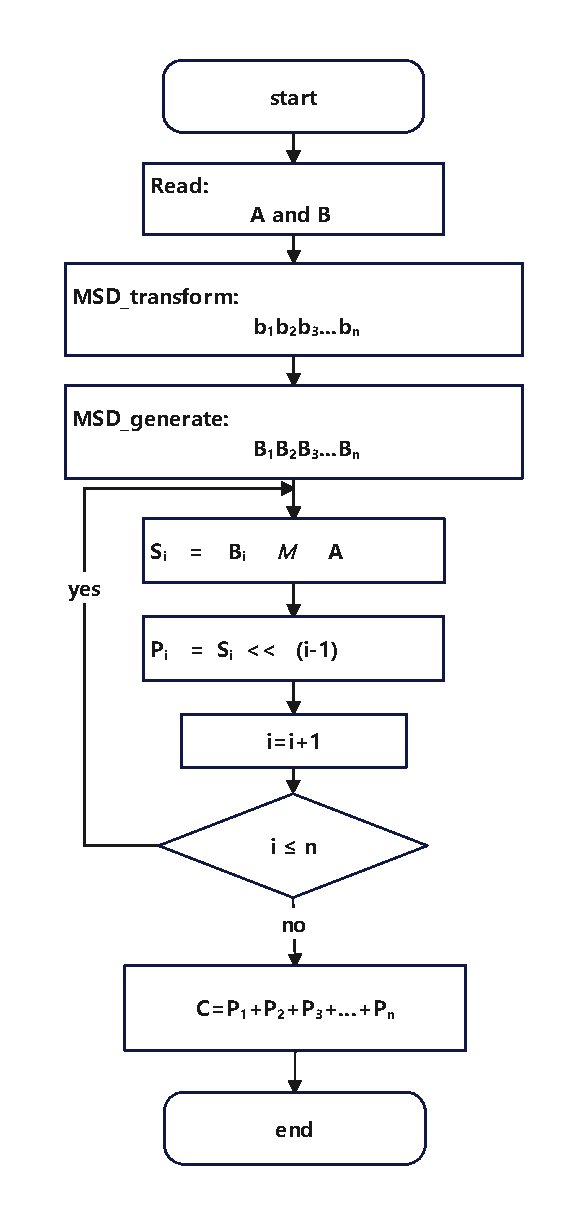
\includegraphics[scale=0.55]{./images/8.pdf}
   % \captionsetup{justification=centering} 
    \caption{RFLMR flowchart}
    \label{fig9}
\end{figure}
In the design process of the RFLMR, we adopted a modular strategy and deeply optimized the transformations of \textit{M}, \textit{T}, \textit{W}, \textit{T’}, and \textit{W’}. Each module undertakes specific encoding conversion tasks, including but not limited to the \textit{M} transformation module (S operator), \textit{T} transformation module (Y operator), \textit{W} transformation module (F operator), \textit{T’} transformation module (J operator), \textit{W’} transformation module (I operator), and an additional $T_2$ transformation module (N operator). The extensive library of electronic logic units on the ALinx 7020 platform (up to thousands) is sufficient to support the parallel deployment of dozens of such essential processors, meaning that only a few operational instructions are needed to complete complex computational tasks efficiently. For instance, a basic module with a processing capacity of 1024 bits in application-oriented scenarios is sufficient to construct five similar architecture processors. Therefore, the RFLMR processor can handle multiple computational tasks simultaneously with just one multiplication instruction call, significantly reducing the repeated execution of operational instructions and saving valuable computation time and hardware resources. This design approach substantially improves computational efficiency and efficiently utilizes hardware resources, bringing unprecedented speed and performance improvements to multiplication operations. The four-valued logic multiplication routine processor, with its unique parallel processing capability and high adaptability, demonstrates advantages in diverse application fields, indicating that it will play a more critical role in the future development of computing technology.
\begin{figure}[H]
 %   \centering
    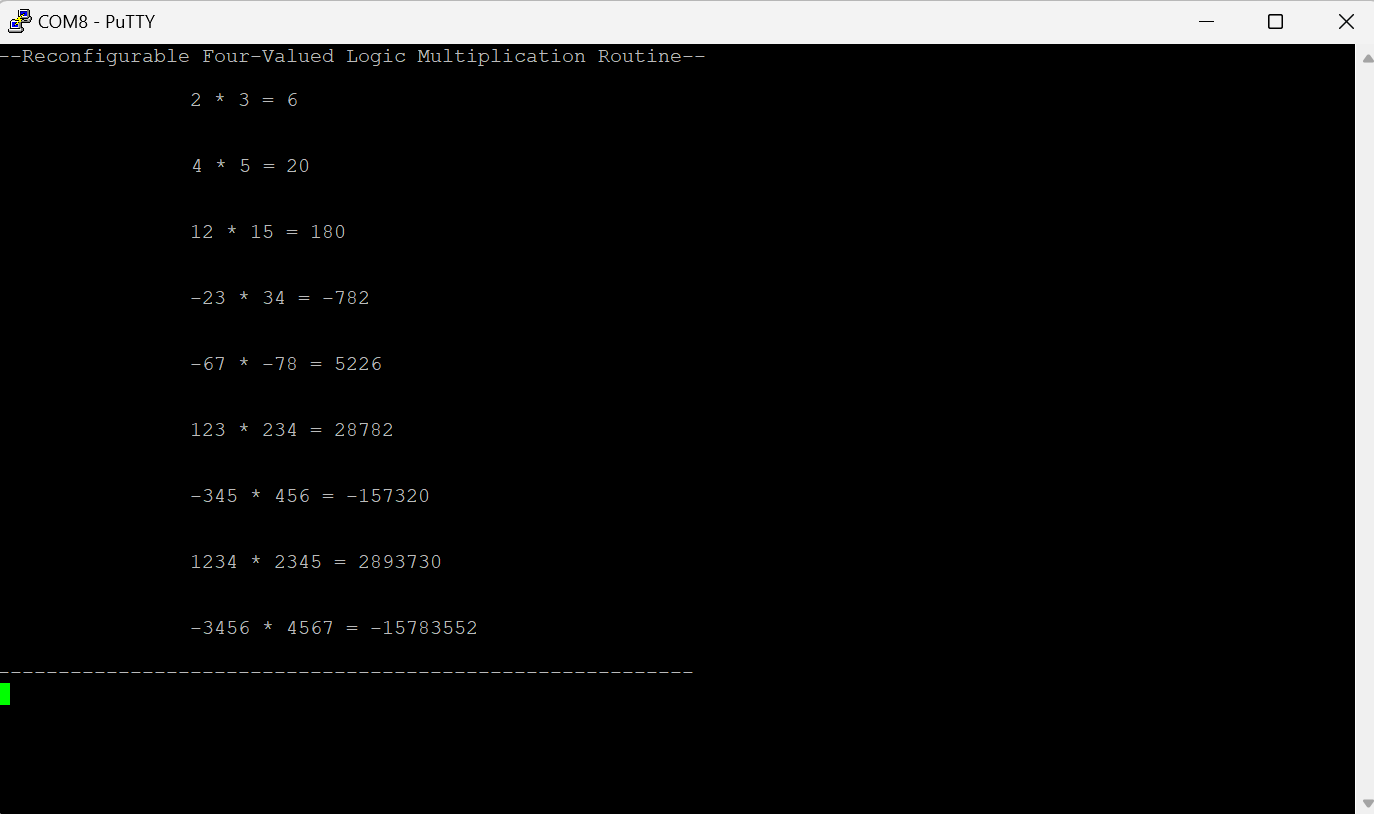
\includegraphics[scale=0.4]{./images/9.png}
  %  \captionsetup{justification=centering} 
    \caption{Putty output results of RFLMR}
    \label{fig8}
\end{figure}
Given that the bit-width of the processor for the RFLMR is set to 33 bits, and each of the three-valued states stored in the register—namely 00, 01, and 10—requires two bits per state, the total register capacity must accommodate 66 bits. To simplify the visual representation, we converted the three-valued states in the register into a more compact MSD numerical representation. Table 7 and Figure 9 show that the experimental results align with the expected outcomes, validating the method’s effectiveness.
To further confirm the accuracy of the results obtained during partial cumulative addition operations, we introduced the Digital Direct Synthesis (DDS) waveform as a verification tool. As an advanced waveform synthesis method, DDS technology can generate signals of arbitrary frequencies, providing significant advantages in verifying the correctness of computational logic. Specifically, taking Examples 1 and 2 as cases, their theoretical expected values are detailed in Table \ref{tab6}. The DDS waveform displays the MSD numbers formed by the conversion. In Example 1 (as shown in Figure \ref{fig10}(\subref{fig10-sub1}), the values in registers \textit{m1} and \textit{m2} match the partial product values transformed by the M(S operator), and the s register outputs the result. In Example 2 (as shown in Figure \ref{fig10}(\subref{fig10-sub2}), the values in registers \textit{m1},\textit{ m2}, and \textit{m3} match the three partial products transformed by the \textit{M}(S operator), thus confirming the correctness of the results.

\begin{figure}[H]
 % \centering
%  \captionsetup{justification=centering} 
  \captionsetup[subfigure]{justification=centering} 
  \begin{subfigure}[b]{0.47\textwidth}
    \centering
    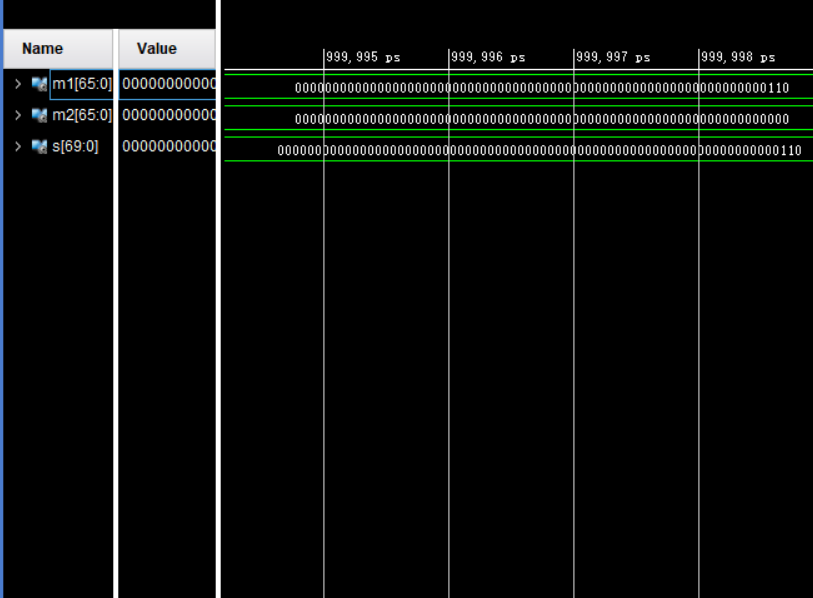
\includegraphics[width=\textwidth]{images/12.png}
    \caption{}
    \label{fig10-sub1}
  \end{subfigure}
  \hfill
  \begin{subfigure}[b]{0.48\textwidth}
    \centering
    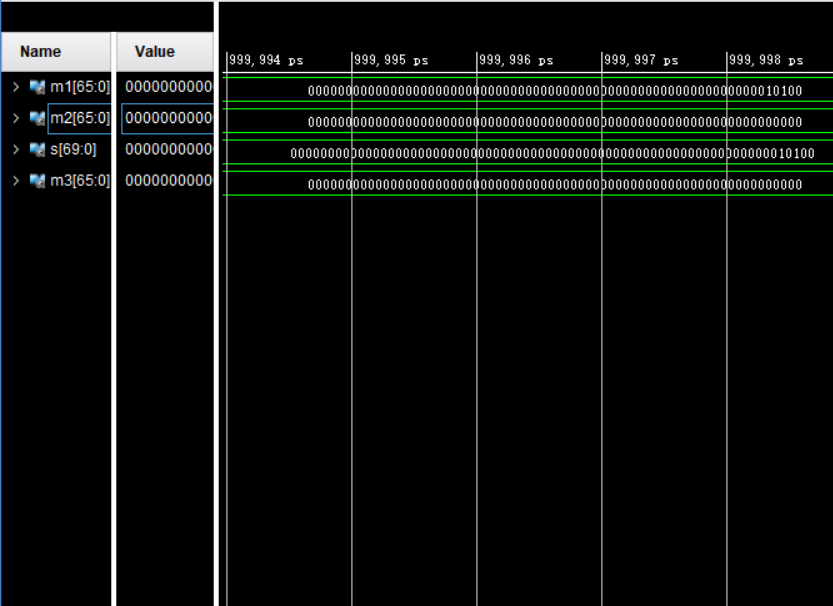
\includegraphics[width=\textwidth]{images/11.png}
    \caption{}
    \label{fig10-sub2}
  \end{subfigure}
    \caption{RFLMR partial product summation DSS waveforms} % 整个图的标题
  \label{fig10}
\end{figure}
\section{Conclusions}
This paper establishes a multiplication routine for a four-valued electronic logic processor. The routine generates partial products through \textit{M} transformation in four-valued logic. Then, it uses the JW-MSD parallel adder to sum the partial products, ultimately completing the design of the multiplication routine. The effectiveness of the multiplication routine was verified through experiments. The constructed multiplication routine lays the foundation for the transition of the four-valued logic electronic processor from laboratory research to applied research. It provides a new approach and method for handling large-number multiplications. The experiments also demonstrated the flexibility and scalability of the reconfigurable four-valued logic processor. By leveraging its reconfigurable characteristics, the RFLMR processor can dynamically adjust its computational functions to improve efficiency when handling complex operations. In the experiments, we rigorously verified each step of the computation of the RFLMR processor through register analysis and serial port debugging tools, ensuring the accuracy of data storage and processing. Particularly in operations involving large numerical ranges, the RFLMR can still be handled efficiently, and the output results meet theoretical expectations. This further demonstrates the potential of the RFLMR in high-performance computing, which can meet the needs of various complex applications and provide strong support for developing future efficient computing technologies.

\authorcontributions{Proposing Reconfigurable Four-Valued Logic Multiplication Routines, S.L.; Determining Computational Data and Validating Experimental Results, X.G. and L.L.; Designing and Constructing Multiplication Routines, S.L. and X.L; Writing-Preliminary Draft Preparation, S.L. and X.L; Writing-Reviewing and Editing, S.L. and S.L.; Supervision, S.Z.; All authors have read and agree to the published version of the manuscript.}

\funding{This work was supported by the National Science Foundation of China (62302307, 62105207, 61866006), the Open Research Fund of Guangxi Key Lab of Human-machine Interaction and Intelligent Decision (GXHIID2209), and University- level general research project of Shanghai Normal University (SK202121), Hainan Provincial Natural Science Foundation of China under Grant (622MS084), the Education Department of Hainan Province of China (Hnjg2022-90), the General scientific research project of Zhejiang Education Department(Y202352358).}


\dataavailability{The data used to support the findings of this study are available from the corresponding author upon request.} 



\acknowledgments{I want to express my gratitude to Prof. Luqun Li, Mr. Li  and all the members of the Reconfigurable Four-Valued Logic Operator Team at Donghua University for their valuable comments and suggestions on this paper.}



% Only for journal Nursing Reports
%\publicinvolvement{Please describe how the public (patients, consumers, carers) were involved in the research. Consider reporting against the GRIPP2 (Guidance for Reporting Involvement of Patients and the Public) checklist. If the public were not involved in any aspect of the research add: ``No public involvement in any aspect of this research''.}

% Only for journal Nursing Reports
%\guidelinesstandards{Please add a statement indicating which reporting guideline was used when drafting the report. For example, ``This manuscript was drafted against the XXX (the full name of reporting guidelines and citation) for XXX (type of research) research''. A complete list of reporting guidelines can be accessed via the equator network: \url{https://www.equator-network.org/}.}

% Only for journal Nursing Reports
%\useofartificialintelligence{Please describe in detail any and all uses of artificial intelligence (AI) or AI-assisted tools used in the preparation of the manuscript. This may include, but is not limited to, language translation, language editing and grammar, or generating text. Alternatively, please state that “AI or AI-assisted tools were not used in drafting any aspect of this manuscript”.}



\conflictsofinterest{The authors state that we have no conflicts of interest. We confirm that there are no financial, personal, or professional affiliations that could be perceived as influencing the research presented in this paper.} 
%\newpage
%%%%%%%%%%%%%%%%%%%%%%%%%%%%%%%%%%%%%%%%%%

%%%%%%%%%%%%%%%%%%%%%%%%%%%%%%%%%%%%%%%%%%
%%% Optional
%\appendixtitles{no} % Leave argument "no" if all appendix headings stay EMPTY (then no dot is printed after "Appendix A"). If the appendix sections contain a heading then change the argument to "yes".
%\appendixstart
%\appendix






%%%%%%%%%%%%%%%%%%%%%%%%%%%%%%%%%%%%%%%%%%
\begin{adjustwidth}{-\extralength}{0cm}

\reftitle{References}

\begin{thebibliography}{999}

\bibitem[Zhang et~al.(2023)]{ref1}
Zhang, S.; Chen, J.; Liu, Z.; Wang, X.; Zhang, C.; Yang, J.
\newblock Key theories and technologies and implementation mechanism of
  parallel computing for ternary optical computer.
\newblock {\em \textit{PloS one}} {\bf \textbf{2023}}, {\em 18},~e0284700.

\bibitem[Wang et~al.(2023)]{ref2}
Wang, S.; Jiang, J.; Wang, Z.
\newblock Research of Tri-State Optical Signal Detectors for Ternary Optical
  Computers.
\newblock {\em \textit{Applied Sciences}} {\bf \textbf{2023}}, {\em 13},~98.

\bibitem[Wang and Shen(2021)]{ref3}
Wang, Z.; Shen, Y.
\newblock Design and implementation of bitwise parallel MSD square rooting in
  ternary optical computer.
\newblock {\em \textit{Optical Engineering}} {\bf \textbf{2021}}, {\em
  60},~085107.

\bibitem[Zhehe et~al.(2023)]{ref4}
Zhehe, W.; Yunfu, S.; Shuang, L.; Honghong, Z.; Jiabao, J.; Chunteng, W.
\newblock Design and Implementation of a Ternary Optical Computer Simulator.
\newblock {\em \textit{Computer Application Research}} {\bf \textbf{2023}},
  {\em 40},~1137--1141.

\bibitem[Shuang et~al.(2019)]{ref5}
Shuang, L.; Jiabao, J.; Zhehe, W.; Honghong, Z.
\newblock Basic theory and key technology of programming platform of ternary
  optical computer.
\newblock {\em \textit{Optik}} {\bf \textbf{2019}}, {\em 178},~327--336.

\bibitem[Yi(2007)]{ref6}
Yi, J.
\newblock Management strategy of data bits in ternary optical computer.
\newblock {\em \textit{Journal of Shanghai University (Natural Science
  Edition)}} {\bf \textbf{2007}}, {\em 13},~519--523.

\bibitem[Sulan et~al.(2018)]{ref7}
Sulan, Z.; Junjie, P.; Yunfu, S.; Xianchao, W.
\newblock Programming model and implementation mechanism for ternary optical
  computer.
\newblock {\em \textit{Optics Communications}} {\bf \textbf{2018}}, {\em
  428},~26--34.

\bibitem[Wang et~al.(2021)]{ref19}
Wang, H.; Ouyang, S.; Shen, Y.; Chen, X.
\newblock Ternary optical computer: an overview and recent developments.
\newblock In Proceedings of the 2021 12th International Symposium on Parallel
  Architectures, Algorithms and Programming (PAAP). IEEE,  \textbf{2021}, pp.
  82--87.

\bibitem[Jin et~al.(2023)]{ref21}
Jin, Y.; Zhang, H.; Chen, X.; Wang, S.; Ouyang, S.; Shen, Y.; Jiang, J.
\newblock Theory and Structure of the Ternary Logic Optical Processor SD16.
\newblock {\em \textit{Journal of Electronics}} {\bf \textbf{2023}}, {\em
  51},~1154--1162.

\bibitem[Jiang et~al.(2021)]{ref22}
Jiang, J.; Zhang, X.; Shen, Y.; Ouyang, S.; Zhou, S.; Peng, J.; Liu, Y.; Jin,
  Y.
\newblock Design and Implementation of the SJ-MSD Adder in Ternary Optical
  Computers.
\newblock {\em \textit{Journal of Electronics}} {\bf \textbf{2021}}, {\em
  49},~275.

\bibitem[Jin et~al.(2019)]{ref23}
Jin, Y.; Wang, Z.; Liu, Y.; Ouyang, S.; Shen, Y.; Peng, J.
\newblock Ternary Optical Computers.
\newblock {\em \textit{Journal of Nature}} {\bf \textbf{2019}}, {\em
  41},~207--218.

\bibitem[Wang et~al.(2023)]{ref24}
Wang, Z.; Shen, Y.; Li, S.; Zhang, H.; Jiang, J.; Wang, C.
\newblock Design and Implementation of the Ternary Optical Computer Simulator.
\newblock {\em \textit{Application Research of Computers}} {\bf \textbf{2023}},
  {\em 40}.

\bibitem[Jin et~al.(2022)]{ref8}
Jin, Y.; Ouyang, S.; Pan, Z.; Wang, Y.; Shen, Y.; Peng, J.; Zhou, S.; Liu, Y.;
  Chen, X.
\newblock A Multi-Digit, Groupable, and Reconfigurable Multi-Valued Electronic
  Calculator and Method.
\newblock CN201811567284.7,  7 \textbf{2022}.

\bibitem[Lu et~al.(2023)]{ref9}
Lu, Y.; Wang, H.; Huang, J.; Zhou, X.; Wu, Y.
\newblock Demonstration system of reconfigurable multi-valued logic electronic
  processor.
\newblock In Proceedings of the Second International Conference on Electronic
  Information Technology (EIT 2023). SPIE,  \textbf{2023}, Vol. 12719, pp.
  190--196.

\bibitem[Sasao and Nakahara(2007)]{ref10}
Sasao, T.; Nakahara, H.
\newblock Implementations of reconfigurable logic arrays on FPGAs.
\newblock In Proceedings of the 2007 International Conference on
  Field-Programmable Technology. IEEE,  \textbf{2007}, pp. 217--223.

\bibitem[Wang et~al.(2021)]{ref11}
Wang, H.; Wu, Y.; Ouyang, S.; Chen, X.; Shen, Y.; Jin, Y.
\newblock The design and implementation of reconfigurable quaternary logic
  processor.
\newblock In Proceedings of the International Conference on Parallel and
  Distributed Computing: Applications and Technologies. Springer,
  \textbf{2021}, pp. 142--149.

\bibitem[Lu et~al.(2023)]{ref12}
Lu, Y.; Wang, H.; Huang, J.; Zhou, X.; Wu, Y.
\newblock Demonstration system of reconfigurable multi-valued logic electronic
  processor.
\newblock In Proceedings of the Second International Conference on Electronic
  Information Technology (EIT 2023). SPIE,  \textbf{2023}, Vol. 12719, pp.
  190--196.

\bibitem[Yan(2010)]{ref13}
Yan, J.
\newblock Design Theory for Devaluation.
\newblock PhD thesis, Shanghai University,  \textbf{2010}.

\bibitem[Yan et~al.(2008)]{ref14}
Yan, J.; Jin, Y.; Zuo, K.
\newblock Design Theory for Devaluation of No-Carry (Borrow) Calculator and Its
  Application in Ternary Optical Computers.
\newblock {\em \textit{Science in China Series E: Technological Sciences}} {\bf
  \textbf{2008}}, {\em 38},~11.

\bibitem[Bocker et~al.(1986)]{ref15}
Bocker, R.P.; Drake, B.L.; Lasher, M.E.; Henderson, T.B.
\newblock Modified signed-digit addition and subtraction using optical symbolic
  substitution.
\newblock {\em \textit{Applied Optics}} {\bf \textbf{1986}}, {\em
  25},~2456--2457.

\bibitem[Peng et~al.(2012)]{ref16}
Peng, J.; Shen, R.; Jin, Y.; Shen, Y.; Luo, S.
\newblock Design and implementation of modified signed-digit adder.
\newblock {\em \textit{IEEE Transactions on Computers}} {\bf \textbf{2012}},
  {\em 63},~1134--1143.

\bibitem[Drake et~al.(1986)]{ref17}
Drake, B.L.; Bocker, R.P.; Lasher, M.E.; Patterson, R.H.; Miceli, W.J.
\newblock Photonic computing using the modified signed-digit number
  representation.
\newblock {\em \textit{Optical Engineering}} {\bf \textbf{1986}}, {\em
  25},~38--43.

\bibitem[Qi et~al.2023)]{ref18}
Qi, B.; Sun, S.; Tong, Y.; Zhang, J.; Wang, Z.; Wang, X.
\newblock Algorithm-based Study on Transformation Combination for Carry-free
  Modified Signed Digit (MSD) Addition.
\newblock In Proceedings of the 2023 IEEE 10th International Conference on
  Cyber Security and Cloud Computing (CSCloud)/2023 IEEE 9th International
  Conference on Edge Computing and Scalable Cloud (EdgeCom). IEEE,
  \textbf{2023}, pp. 298--304.

\bibitem[Jin et~al.(2011)]{ref20}
Jin, Y.; Shen, Y.; Peng, J.; Xu, S.; Ding, G.; Yue, D.; You, H.
\newblock Theory and Structure of the MSD Adder in Ternary Optical Computers.
\newblock {\em \textit{Science China Information Sciences}} {\bf
  \textbf{2011}}, {\em 41},~541--551.

\end{thebibliography}


%
%\externalbibliography{yes}
%\bibliography{references.bib}
%\printbibliography
%\bibliography{references.bib}
\PublishersNote{}
\end{adjustwidth}
\end{document}

